\documentclass[12pt,notitlepage]{report}
\usepackage[algoruled, noend]{algorithm2e}
\usepackage{a4wide}
\usepackage{graphicx}
\usepackage[left=4cm]{geometry} % okraje
\usepackage{latexsym}% kvuli symbolum v grafech vkladanych z gnuplotu
\usepackage{amsfonts}
\usepackage{amssymb,amsmath}
\usepackage[cp1250]{inputenc}
\usepackage[czech,english]{babel}
\usepackage[T1]{fontenc}
\usepackage{listings}
\usepackage{subfigure}
\selectlanguage{english}
\usepackage{verbatim}
\usepackage{enumerate}
\usepackage{color}
\usepackage{float}
\usepackage{epsfig}

\lstset{language=C++, basicstyle=\scriptsize, commentstyle=, showstringspaces=true} 

\title{Adaptive hp Discontinuous Galerkin Method
for Nonstationary Compressible Euler Equations} 
\author{Luk� Korous} 
\renewcommand{\sectionmark}[1]{\markright{#1}{}}

\frenchspacing
\pagenumbering{arabic}
\oddsidemargin  0.3in	% levy okraj stranky; pripocte se 1 inch
\evensidemargin 0.2in	% pravy okraj stranky; pripocte se 1 inch
\textwidth      5.8in	% sirka textu
\headheight     0.0in	% vyska hlavicky
\topmargin      0.2in	% horni okraj
\textheight     8.5in	% vyska textu

\begin{document}

\include{commands}

\begin{titlepage}
    \begin{center}
        
        \vspace*{3em}
        \textsc{\LARGE University of West Bohemia in Pilsen}\\[0.5em]
        \textsc{\LARGE Faculty of Electrical Engineering}\\[5em]
        
        {\Large Doctoral thesis}\vspace*{1em}
        \rule{\linewidth}{0.5mm}
        \\[1em]
        {\huge \textsc{Large-scale Numerical Simulations of Magneto-Hydrodynamics Phenomena in Astrophysics} \\[0.4cm]}
        \rule{\linewidth}{0.5mm}
        \\[3em]
        
        {\Large Mgr. Luk� \textsc{Korous}}
				\end{center}
				\ \\ TODO
				\\ - popsat numerical flux, ze je non-differentiable, ze se vyhodnocuje na hranach a ze to je challenging z pohledu adaptivity, paralelismu a periodickych podminek
				\\ - obecne MHD num fluxy, kolik je tam vlastnich cisel, cili kolik mezistavu, jake jsou ruzne toky a proc se nepouziva presny resic
				\\ - HLLD, presny popis, proc ne ten flux s jeste vice stavy (drahy)
				\\\ 
				\\ do uvodu napsat vice o state-of-the-art, odkaz na Mirovo clanek, ukazat tam ty FD vysledky, ze je chceme nahradit a ze je tam hodne dulezita adaptivity
				\\ pak teda popsat az tam z toho budu davat vysledky, tak vykopirovat nejaky rovnice IC / BC z clanku, jak se to implementuje, atd.
				\\ srovnani
				\\\ 
				\\ adaptivita - ukazat na 2d prikladu z Hermesu co to je referencni reseni, co to je ||zprojektovane - presne|| (v dealu?), co to je tohle bez normy, zminka o distribuovanosti, ze musim napocitat nejaky thresholdy mapReducem, atd.
				\\ napsat pak algoritmus tedy cely, kde je casovy krok, adaptivita (ze se vraci casovy krok po zjemneni / zhrubeni, aby se neztracela informace), atd.
				\\ \ \\
				\\ popis a vysledky Blastu, O-T
				\\ - odkazy na clanky, popis
				\\ - bez adaptivity jen "pocita to"
				\\ - s adaptivitou "a navic tak presne to spoctu a usetrim 80\% dofu"
				\\ -- tohle ukazovat na rezech hustotou - bylo by fajn nejaky najit
				\vfill
				\begin{center}
        {\large 2016}
    \end{center}
\end{titlepage}
\chapter*{Abstract}
The objective of this Doctoral Thesis was to develop, implement and test new algorithms for the large-scale solution of nonstationary compressible MHD equations based on higher-order discontinuous Galerkin (DG) methods. The basis for the new methods will be the discontinuous Galerkin methods and adaptive mesh refinement (AMR) algorithms. The new algorithms will be implemented and tested in the framework of the open source library Deal.II, and they will be applied to selected problems of MHD in astrophysics, namely the magnetic reconnection phenomena.

\section*{Keywords}
numerical simulation, finite element method, MHD equations, adaptivity, discontinuous Galerkin method, astrophysics, solar flares, CME, magnetic reconnection

\chapter*{Abstract [CZ]}
TODO

\section*{Keywords [CZ]}
TODO


\chapter*{Acknowledgement}
TODO - prelozit

\chapter*{Statement}
TODO - prelozit

P�edkl�d�m t�mto k~posouzen� tezi dizerta�n� pr�ce, zpracovanou na b�hem doktorsk�ho studia na Fakult� elektrotechnick� Z�pado�esk� univerzity v~Plzni.
\\
\vspace{1em}
\\
Prohla�uji, �e jsem tuto pr�ci vypracoval samostatn�, s~pou�it�m uveden� odborn� literatury, a pramen� a �e ve�ker� software, pou�it� p�i jej�m �e�en� a zpracov�n�, byl vyu�it s~respektov�n�m v�ech jeho licen�n�ch podm�nek.
\\
\vspace{3em}
\\
In Pilsen, \today, Luk� Korous
%%%
\addcontentsline{toc}{chapter}{Introduction}

\begin{flushleft}
{\LARGE{\textbf{{Introduction}}}}
\end{flushleft}

Discontinuous Galerkin methods (DG methods) in mathematics form a class of numerical methods for solving partial differential equations. They combine features of the finite element and the finite volume framework and have been successfully applied to hyperbolic, elliptic and parabolic problems arising from a wide range of applications. DG methods have in particular received considerable interest for problems with a dominant first-order part, e.g. in electrodynamics, fluid mechanics and plasma physics.

Discontinuous Galerkin methods were first proposed and analyzed in the early 1970s as a technique to numerically solve partial differential equations. In 1973 Reed and Hill introduced a DG method to solve the hyperbolic neutron transport equation.

The origin of the DG method for elliptic problems cannot be traced back to a single publication as features such as jump penalization in the modern sense were developed gradually. However, among the early influential contributors were Babu�ka, J.-L. Lions, Nitsche and Zlamal. Interestingly DG methods for elliptic problems were already developed in a paper by Baker in the setting of 4th order equations in 1977. A more complete account of the historical development and an introduction to DG methods for elliptic problems is given in a publication by Arnold, Brezzi, Cockburn and Marini. A number of research directions and challenges on DG methods are collected in the proceedings volume edited by Cockburn, Karniadakis and Shu.

The discontinuous Galerkin (DG) methods are locally conservative, stable, and high-order accurate methods which can easily
handle complex geometries, irregular meshes with hanging nodes, and approximations that have polynomials of different
degrees in different elements. These properties, which render them ideal to be used with hp-adaptive strategies, not only
have brought these methods into the main stream of computational fluid dynamics, for example, in gas dynamics, compressible and incompressible flows, turbomachinery, magneto-hydrodynamics,
granular flows, semiconductor device simulation, etc., but have also prompted their application
to a wide variety of problems for which they were not originally intended like, for example, second-order elliptic problems, and elasticity.

\ \\Some more stuff here, references, etc...

%\addcontentsline{toc}{chapter}{Introduction}
%\begin{flushleft}
%{\LARGE{\textbf{{Introduction}}}}
%\end{flushleft}
%Doplnit
%%%

\chapter{Compressible flow and the Euler equations}
	\section{Equations decribing the flow}
	We consider a time interval $\left(0,T\right)$ and space domain $\Omega_{\textit{t}}\subset \mathbb{R}^3$ occupied by a fluid at time $t$.
	By $\mathcal{M}$ we denote the space-time domain in consideration: 
\begin{equation}\label{M}
 \mathcal{M}=\left\{\left(\textbf{\textit{x}},t\right);\\\textbf{\textit{x}}\in\Omega_{\textit{t}},t\in\left(0,T\right)\right \}.
\end{equation}
	Moreover we assume that $\mathcal{M}$ is an open set.
\subsection{Description of the flow}
\paragraph{}
In Computational Fluid Dynamics there exist two classical approaches to the description of the flow, the \textit{Lagrangian description} and the \textit{Eulerian description}.
\paragraph{}

The idea of the Lagrangian description is to monitor each fluid particle along its pathline (i.e. the curve which the particle traverses in time).
If we wanted to set a computational mesh using this description, it would mean to firmly connect nodes of the mesh with certain particles (i.e. the node and the particle would have to share their space coordinates) and move the mesh accordingly to the motion of the fluid as to preserve the node - corresponding particle connection at each time instant.
The obvious drawback is the necessity to perform re-meshing operations very frequently, especially when dealing with large distortion of the fluid.
\paragraph{}

The Eulerian description focuses on fluid particles that move through fixed points within a computational domain. In other words, whereas in the Lagrangian description the particle was fixed and the point in space it was currently occupying was changing, now it is the point in space that holds still and the particle in consideration is changing and is always corresponding to the one that is currently occupying the considered point in space. From this idea it follows that a computational mesh for this description would be fixed with respect to time.
\paragraph{}
It is not difficult to imagine that formulation of some basic mechanical principles could be easier for the moving particle, that is using the Lagrangian approach.
However, the Eulerian description is used for the formulation of conservation laws as will be seen in the following subsections.
Last, using this approach, large distortions of fluid domain can be handled with relative ease.
\paragraph{}
We shall proceed now with basics of the Lagrangian and the Eulerian descriptions and their relation. We shall present the equations describing the flow derived from conservation laws in their integral forms using the Eulerian approach.
\paragraph{Lagrangian description}\ \\
We specify the particle in consideration using the mapping 
\begin{equation}\label{phi_def}
\bsm{\varphi}\left(\bs{X},t_0;t\right)
\end{equation} 
which determines the current (at time $t$) position $\bs{x}\in\Omega_t$ of the particle that occupies the point $\bs{X}$ at time $t_0$, i.e.
\begin{equation}\bs{x} = \bsm{\varphi}\left(\bs{X},t_0;t\right),\ \bs{X}\in\Omega_{t_0},
\end{equation}
where we can omit the reference time $t_0 $ and write
\begin{equation}\label{x=phi}
\bs{x} = \bsm{\varphi}\left(\bs{X},t\right).
\end{equation}
Customarily the components $X_1,X_2,X_3$ of the reference point $\bs{X}$ are called the \textit{Lagrangian coordinates} and the components
$x_1,x_2,x_3$ of the point $\bs{x}$ in the current configuration $\Omega_t$ are called the \textit{Eulerian coordinates}. The \textit{velocity} and \textit{acceleration} of the particle given by the reference point $\bs{X}$ are defined as
\begin{equation}\label{v_def}
\hat{v}\left(\bs{X},t\right) = \pds{\bsm{\varphi}}{t}\left(\bs{X},t_0;t\right),
\end{equation}
\begin{equation}
\hat{a}\left(\bs{X},t\right) = \frac{\partial^2{\bsm{\varphi}}}{\partial{t}^2}\left(\bs{X},t_0;t\right),
\end{equation}
provided the above derivatives exist.
\paragraph{Eulerian description}\ \\
Using once again the mapping $\phib$ defined in~\eqref{phi_def}, relation~\eqref{x=phi} and the Lagrangian definition of velocity~\eqref{v_def}, we can express the \textit{velocity} of the fluid particle passing through the point $\bs{x}$ at time $t$: 
\begin{equation}
\bs{v}\left(\bs{x},t\right) = \hat{\bs{v}}\left(\bs{X},t\right) = \pds{\bsm{\varphi}}{t}\left(\bs{X},t\right),
\end{equation}
where $\bs{x} = \phib\left(\bs{X},t\right).$ \\
We shall demand the following regularity from the velocity function:
\begin{equation}\label{v_reg}
\bs{v}\in\left[\mathcal{C}^1\left(\mathcal{M}\right)\right]^3.
\end{equation}
We can pass to the Eulerian coordinates from the Lagrangian ones by solving the following initial value problem:
\begin{equation}\label{lagrange-euler}
 \pds{\bs{x}}{t} = \bs{v}\left(\bs{x},t\right),\ \ \bs{x}\left(t_0\right) = \bs{X}.
\end{equation}
Under assumption~\eqref{v_reg}, the problem~\eqref{lagrange-euler} has exactly one maximal solution $\phib\left(\bs{X},t_0,t\right)$ for each $\left(\bs{X},t_0\right)\in\mathcal{M}$ defined for $t$ from a certain subinterval of $\left(0,T\right)$. Moreover, in its domain of definition, the mapping $\phib$ has continuous first order derivatives with respect to $X_1,\ X_2,\ X_3,\ t_0,\ t$ and continuous second order derivatives $\partial^2\phib/\partial{t}\partial{X_i}$, $\partial^2\phib/\partial{t_0}\partial{X_i}$, $i = 1,\ 2,\ 3$. These statements result from theory of classical solutions of ordinary differential equations.
\paragraph{}
Under assumption~\eqref{v_reg}, the \textit{acceleration} of the particle passing through the point $\bs{x}$ at time $t$ can be expressed as 
\begin{equation}
 \bs{a}\left(\bs{x},t\right) = \pds{\bs{v}}{t}\left(\bs{x},t\right) + \sum_{i=1}^{3}v_i\left(\bs{x},t\right)\pds{\bs{v}}{x_i}\left(\bs{x},t\right).
\end{equation}
This, written in a short form reads
\begin{equation}\label{a_def_2}
 \bs{a}= \pds{\bs{v}}{t} + \left(\bs{v}\cdot\mathsf{grad}\right)\bs{v} = \pds{\bs{v}}{t}+\left(\bs{v}\cdot\nabla\right)\bs{v},
\end{equation}
where the differentiation represented by the symbol $\nabla$ is with respect to the spatial variables $x_1,x_2,x_3$.

\subsection{The Transport theorem}
\paragraph{}
We wish to study some physical quantity which is transported by fluid particles in our space-time domain $\mc{M}$.
Let a function $F = F\left(\bs{x},t\right):\mathcal{M}\longrightarrow \mathbb{R} $ represent some physical quantity in the Eulerian coordinates, and let us consider a system of fluid particles filling a bounded domain $\mathcal{V}\lo{t}\ro \subset \Omega_{t}$ at time $t$. By $\mathcal{F}$ we denote the total amount of the quantity represented by the function $F$ contained in $\mc{V}\lo{t}\ro $:
\begin{equation}
 \mathcal{F}\left(t\right) = \int_{\mathcal{V}\left(t\right)}F\left(\bs{x},t\right)d\bs{x}.
\end{equation}
For the formulation of fundamental equations describing the flow we need to calculate the rate of change of the quantity $\mc{F}$ bound on the system of particles considered. In other words we shall be interested in the derivative
\begin{equation}\label{f_der}
 \d{\mathcal{F}\left(t\right)}{t}=\d{}{t}\int_{\mathcal{V}\left(t\right)}F\left(\bs{x},t\right)d\bs{x}.
\end{equation}
In the following we shall suppose that~\eqref{v_reg} holds.
\paragraph{Lemma 1.1}
\itshape
\ \newline
Let $t_0 \in\left(0,T\right), \mathcal{V}\left(t_0\right)$ be a bounded
 domain and let $\overline{\mathcal{V}\left(t_0\right)}\subset\Omega_{\textit{t}_0}$.
Then there exist an interval $\left(t_1,t_2\right)\subset\left(0,T\right)$, $t_0\in\left(t_1,t_2\right)$ such that the following conditions are satisfied:
\renewcommand{\labelenumi}{\alph{enumi})}
\begin{enumerate}
\upshape
 \item\itshape The mapping '$t\in\left(t_1,t_2\right), \bs{X}\in\mathcal{V}\left(t_0\right)\longrightarrow\bs{x}=\bsm{\varphi}\left(\bs{X},t_0;t\right)\in\mathcal{V}\left(t\right)$' has continuous first order derivatives with respect to $t,X_1,X_2,X_3$ and continuous second order derivatives 
${\partial^2\bsm{\varphi}}/{\partial{t}\partial{{X}_i}},\ i = 1, 2, 3.$
\upshape
 \item\itshape The mapping '$\bs{X}\in\mathcal{V}\left(t_0\right)\longrightarrow\bs{x}= \bsm{\varphi}\left(\bs{X},t_0;t\right)\in\mathcal{V}\left(t\right)$' is for all ${t}\in\left(t_1,t_2\right)$ a continuously differentiable one-to-one mapping of $\mathcal{V}\left(t_0\right)$ onto $\mathcal{V}\left(t\right)$ with continuous and bounded Jacobian $\mc{J}\left(\bs{X},t\right)$ which satisfies the condition 
$$
\mc{J}\left(\bs{X},t\right) > 0\ \ \forall\bs{X}\in \mathcal{V}\left(t_0\right),\ \forall{t}\in\left(t_1,t_2\right).$$
 \upshape
 \item\itshape The inclusion $$
\left\{\left(\bs{x},t\right);\ t\in\left[t_1,t_2\right], \bs{x}\in \overline{{\mathcal{V}\left(t\right)}}\right\}\subset\mathcal{M}$$
holds and therefore the mapping \bs{v} has continuous and bounded first order derivatives on $\left\{\left(\bs{x},t\right);\ t\in\left(t_1,t_2\right), \bs{x}\in\mathcal{V}\left(t\right)\right\}$ with respect to all variables.
\upshape
 \item\itshape $\bs{v}\left(\bsm{\varphi}\left(\bs{X},t_0;t\right),t\right)=\pds{\bsm{\varphi}}{t}\left(\bs{X},t_0;t\right)\ \forall\bs{X}\in\mathcal{V}\left(t_0\right),\ \forall\ t\in\left(t_1,t_2\right).$
\end{enumerate}
\upshape
For proof, see~\cite{1993}.
\paragraph{Theorem 1.2 - The transport theorem}
\ \newline
\itshape
Let conditions from Lemma 1.1, a)-d) be satisfied and let the function $F = F\left(\bs{x},t\right)$ have continuous and bounded first order derivatives on the set \\$\left\{\left(\bs{x},t\right);t\in\left(t_1,t_2\right),\,x\in\mathcal{V}\left(t\right)\right\}$. Let $\mc{F}\lo{t}\ro = \int_{\mathcal{V}\left(t\right)}F\left(\bs{x},t\right) d\bs{x}$.
\\
Then for each $t\in\left(t_1,t_2\right)$ there exists a finite derivative
\begin{eqnarray}
\nonumber\frac{d\mathcal{F}}{dt}\left({t}\right)
& = &
\frac{d}{dt}\int_{\mathcal{V}\left(t\right)}F\left(\bs{x},t\right) d\bs{x}
 \\
& = & \int_{\mathcal{V}\left(t\right)}
	\left[
		\pds{F}{t}\left(\bs{x},t\right)
		+
		\mathrm{div}\left(F\bs{v}\right)\left(\bs{x},t\right)\right] d\bs{x}.
\end{eqnarray}\upshape
For proof, see~\cite{compress}.
\subsection{The continuity equation}
\ \newline
The \textit{density of fluid is} a function
$$\rho:\mathcal{M} \longrightarrow \left(0,+\infty\right)$$
which allows us to determine the mass $m\left(\mathcal{V};t\right)$ of the fluid contained in any subdomain $\mathcal{V}\subset\Omega_{\textit{t}}:$
\begin{equation}\label{m}
 m\left(\mathcal{V};t\right) = \int_{\mathcal{V}}\rho\left(\bs{x},t\right)d\bs{x}.
\end{equation}
\paragraph{Assumptions 1.3}\label{assumption}\ \\
In what follows, let $\rho\in\mathcal{C}^1\lo{}\mc{M}\ro $ and as before let $\bs{v}\in\left[\mathcal{C}^1\left(\mathcal{M}\right)\right]^3$. We shall consider an arbitrary time instant $t_0 \in\left(0,T\right)$ and a moving piece of fluid formed by the same particles at each time instant and filling at time $t_0$ a bounded domain $\mathcal{V}\subset\overline{\mathcal{V}}\subset\Omega_{{t}_0}$ with a Lipschitz-continuous boundary $\partial\mathcal{V}$ called the \textit{control volume} in the domain $\Omega_{{t}_0}$. By $\mc{V}\lo{t}\ro $ we denote the domain occupied by this piece of fluid at time $t\in\lo{}t_1,t_2\ro $, where $\lo{}t_1,t_2\ro $ is a sufficiently small interval containing $t_0$ with properties from Lemma 1.1.
\paragraph{}Since the domain $\mathcal{V}\left(t\right)$ is formed by the same particles at each time instant, the \textit{conservation of mass} can be formulated in the following way:
\textit{The mass of the piece of fluid represented by the domain }$\mathcal{V}\left(t\right)$\textit{ does not depend on time t.} This means that
\begin{equation}
 \d{m\left(\mathcal{V}\left(t\right);t\right)}{t} = 0,\ t \in\left(t_1,t_2\right),
\end{equation}
where with respect to~\eqref{m} we have
\begin{equation}\label{mass}
 m\left(\mathcal{V}\left(t\right);t\right)=\int_{\mathcal{V}\lo{t}\ro}\rho\left(\bs{x},t\right)d\bs{x}.
\end{equation}
From Theorem 1.2 for a function $F:=\rho$ we get the identity
\begin{equation}
\int_{\mathcal{V}\left(t\right)}\left[\pds{\rho}{t}\left(\bs{x},t\right) + \mathrm{div}\left(\rho\bs{v}\right)\left(\bs{x},t\right)\right] d\bs{x} = 0,\ \ t\in\left(t_1,t_2\right).
\end{equation}
If we substitute $t:=t_0$ and take into account that $\mathcal{V}\left(t_0\right) = \mathcal{V}$, we conclude that
\begin{equation}
\int_{\mathcal{V}}\left[\pds{\rho}{t}\left(\bs{x},t_0\right) + \mathrm{div}\left(\rho\bs{v}\right)\left(\bs{x},t_0\right)\right] d\bs{x} = 0
\end{equation}
for an arbitrary $t_0\in\left(0,T\right)$ and an arbitrary control volume $\mathcal{V}\subset\Omega_{t_0}$. We use the following Lemma in order to derive the differential form of the law of conservation of mass:
\paragraph{Lemma 1.4}\label{4}\ \\
\itshape
Let $\Omega\subset\mathbb{R}^N$ be an open set and let $f\in\mathcal{C}\left(\Omega\right)$. Then the following holds: \\\\
$f\equiv0$ in $\Omega$ if and only if $\int_{\mathcal{V}}f\lo{}\bs{x}\ro\,d\bs{x}=0$ for any bounded open set $\mathcal{V}\subset\overline{\mathcal{V}}\subset\Omega$.
\upshape\paragraph{}
Now we use Lemma 1.4 and obtain the differential form of the law of conservation of mass called the \textit{continuity equation}:
\begin{equation}\label{continuity}
 \pds{\rho}{t}\left(\bs{x},t\right) + \mathrm{div}\left(\rho\left(\bs{x},t\right)\bs{v}\left(\bs{x},t\right)\right) = 0,\ \  \bs{x}\in\Omega_t,\ t\in\left(0,T\right).
\end{equation}
\subsection{The equations of motion}
We proceed by deriving basic dynamical equations describing flow motion from the \textit{law of conservation of momentum} which can be formulated in this way:
\itshape
\paragraph{}
The rate of change of the total momentum of a piece of fluid formed by the same particles at each time and occupying the domain $\mathcal{V}\left(t\right)$ at time instant $t$ is equal to the force acting on $\mathcal{V}\left(t\right).$
\upshape
\paragraph{}
Let assumptions 1.3 be satisfied. The total momentum of particles contained in $\mathcal{V}\left(t\right)$ is given by
\begin{equation}\label{moment_1}
 \bsm{\mathcal{H}}\left(\mathcal{V}\left(t\right)\right)= \int_{\mathcal{V}\left(t\right)}\rho\left(\bs{x},t\right)\bs{v}\left(\bs{x},t\right)d\bs{x}.
\end{equation}
Moreover, denoting by $\bsm{\mathcal{F}}\left(\mathcal{V}\left(t\right)\right)$ the force acting on the volume $\mathcal{V}$, the law of conservation of momentum reads
\begin{equation}\label{moment_2}
 \d{\bsm{\mathcal{H}}\left(\mathcal{V}\left(t\right)\right)}{t}=\bsm{\mathcal{F}}\left(\mathcal{V}\left(t\right)\right),\ \ t\in\left(t_1,t_2\right).
\end{equation}
Using Theorem 1.2 for functions $F:=\rho{v}_i$, $i=1, 2, 3$, we get
\begin{equation}
 \int_{\mathcal{V}\left(t\right)}\left[\pds{}{t}\left(\rho\left(\bs{x},t\right)v_i\left(\bs{x},t\right)\right)+\mathrm{div}
\left(\rho\left(\bs{x},t\right)v_i\left(\bs{x},t\right)\bs{v}\left(\bs{x},t\right)\right)\right]\ d\bs{x}= \mathcal{F}_i\left(\mathcal{V}\left(t\right)\right),
\end{equation}
\begin{equation}
i = 1, 2, 3,\ t\in\left(t_1,t_2\right). \nonumber
\end{equation}
Taking into account that $t_0\in\lo{}0,T\ro $ is an arbitrary time instant and $\mc{V}_{t_0}=\mc{V}\subset\overline{\mc{V}}\subset\Omega_{t_0}$, where $\mc{V}$ is an arbitrary control volume, we get the law of conservation of momentum in the form where we write $t$ instead of $t_0$:
\begin{equation}\label{motion}
  \int_{\mathcal{V}}\left[\pds{}{t}\left(\rho\left(\bs{x},t\right)v_i\left(\bs{x},t\right)\right)+\mathrm{div}
\left(\rho\left(\bs{x},t\right)v_i\left(\bs{x},t\right)\bs{v}\left(\bs{x},t\right)\right)\right]\ d\bs{x}= \mathcal{F}_i\left(\mathcal{V};t\right),\\
\end{equation}
$i$ = 1, 2, 3, for an arbitrary $t\in\left(0,T\right)$ and an arbitrary control volume $\mathcal{V}\subset\overline{\mathcal{V}}\subset\Omega_t$.
\paragraph{}
According to~\cite{1993}, the components $\mathcal{F}_i\left(\mathcal{V};t\right),\,i=1, 2, 3,$ of the vector $\bsm{\mathcal{F}}\left(\mathcal{V};t\right)$ can be expressed as
\begin{equation}
\mathcal{F}_i\left(\mathcal{V};t\right) = \int_{\mathcal{V}}\rho\left(\bs{x},t\right)f_i\left(\bs{x},t\right)dx + \int_{\partial\mathcal{V}}\sum_{j=1}^3\tau_{ji}\left(\bs{x},t\right)n_j\left(\bs{x}\right)dS,\,i = 1,2,3,
\end{equation}
assuming that $\tau_{ij}\in\mc{C}^1\lo{}\mc{M}\ro $ and $f_i\in\mc{C}\lo{}\mc{M}\ro,\ \lo{}i,\,j=1, 2, 3\ro $. Here $\tau_{ji}$ are components of the \textit{stress tensor} $\mc{T}$ and $f_i$ are components of the \textit{density of the volume force} $\bs{f}$.
Substituting this into~\eqref{motion},
we get
\begin{eqnarray}
\int_{\mathcal{V}}\left[\pds{}{t}\left(\rho\left(\bs{x},t\right)v_i\left(\bs{x},t\right)\right)+\mathrm{div}\left(\rho\left(\bs{x},t\right)v_i\left(\bs{x},t\right)\bs{v}\left(\bs{x},t\right)\right)\right]dx= \\
\int_{\mathcal{V}}\rho\left(\bs{x},t\right)f_i\left(\bs{x},t\right)dx + \int_{\partial\mathcal{V}}\sum_{j=1}^3\tau_{ji}\left(\bs{x},t\right)n_j\left(\bs{x}\right)dS,\ \ i = 1,2,3,
\end{eqnarray}
for each $t\in\left(0,T\right)$ and an arbitrary control volume $\mathcal{V}$ in $\Omega_t$.
Moreover, applying Green's theorem and Lemma 1.4, we obtain the desired \textit{equation of motion of a general fluid in the differential conservative form}
\begin{equation}
 \pds{}{t}\left(\rho{v_i}\right)+\mathrm{div}\left(\rho{v_i}\bs{v}\right)=\rho{f_i} + \sum_{j=1}^3\pds{\tau_{ji}}{x_j},\ \ i = 1, 2, 3.
\end{equation}
This can be written as 
\begin{equation}\label{general motion}
 \pds{}{t}\left(\rho\bs{v}\right)+\mathrm{div}\left(\rho\bs{v}\otimes\bs{v}\right) = \rho\bs{f}+\mathrm{div}\,\mathcal{T},
\end{equation}
where $\otimes$ denotes the \textit{tensor product}:
\begin{displaymath}
\bs{a}\otimes\bs{b} =
\left(
\begin{array}{ccc}
a_1b_1 & a_1b_2 & a_1b_3 \\
a_2b_1 & a_2b_2 & a_2b_3 \\
a_3b_1 & a_3b_2 & a_3b_3
\end{array}
\right),
\end{displaymath}
and 
$\mathrm{div}\left(\bs{a}\otimes\bs{b}\right)$ is a vector quantity:
\begin{displaymath}
\mathrm{div}\left(\bs{a}\otimes\bs{b}\right)=
\left(
\begin{array}{ccc}
\displaystyle\sum_{i=1}^{3}\pds{}{x_i}a_ib_1, & \displaystyle\sum_{i=1}^{3}\pds{}{x_i}a_ib_2, & \displaystyle\sum_{i=1}^{3}\pds{}{x_i}a_ib_3
\end{array}
\ro
^T.
\end{displaymath}
\subsection{The Navier-Stokes equations}
\paragraph{}
The relation between the stress tensor and other quantities describing fluid flow, the velocity and its derivatives in particular, represent the so-called \textit{rheological equations} of the fluid. For the derivation of the Navier-Stokes equations we shall use
\begin{equation}\label{tau}
 \mathcal{T} = \left(-p+\lambda\mathrm{div}\bs{v}\right)\mathbb{I}+ 2\mu\mathbb{D}\left(\bs{v}\right),
\end{equation}
where $\mathbb{D}$ is the deformation velocity tensor:
\begin{equation}
\mathbb{D}=\mathbb{D}\lo{}\bs{v}\ro=\lo{}d_{ij}\ro_{i,j=1}^3,\ d_{ij}=\frac12\lo{}\pds{v_i}{x_j}+\pds{v_j}{x_i}\ro,
\end{equation}
$\lambda, \mu$ are constants or scalar functions of thermodynamical quantities, \upshape$\lambda$ and $\mu$ are called the \textit{first} and the \textit{second} \textit{viscosity coefficient} respectively. For the assumptions under which we can write~\eqref{tau} see~\cite{1993}.
Altough viscosity coefficients can be functions of thermodynamical quantities (most important of which is $\theta$, the absolute temperature) we shall treat them as if they were constants. Let assumptions 1.3 be satisfied and let us assume that 
\begin{equation}\label{nav_asu}
\frac{\partial{\bs{v}}}{\partial{t}}\in\left[\mathcal{C}\left(\mathcal{M}\right)\right]^3,\ \frac{\partial^2\bs{v}}{\partial{x_i}
\partial{x_j}}\in\left[\mathcal{C}\left(\mathcal{M}\right)\right]^3\ \left(i,j = 1, 2, 3\right).
\end{equation}
Now let us substitute relation~\eqref{tau} into the general equations of motion~\eqref{general motion} with the assumption of constant viscosity coefficients and assumptions~\eqref{nav_asu}. We come to the Navier-Stokes equations in the form
\begin{equation}\label{Nav-Simple}
\pds{\left(\rho\bs{v}\right)}{t} + \mathrm{div}\left(\rho\bs{v}\otimes\bs{v}\right)= \rho\bs{f} - \nabla\,p +
\mu\,\triangle{\bs{v}} + \lo{}\mu+\lambda\ro\,\nabla\mathrm{div}\,\bs{v}.
\end{equation}
For details see~\cite{compress}.
\subsection{The energy equation}
Now let us derive a differential equation equivalent to the \textit{law of conservation of energy}. As in the preceding subsections, we consider a piece of fluid represented by a control volume $\mathcal{V}\lo{t}\ro $ satisfying assumptions 1.3. The law of conservation of energy can be formulated as follows:
\itshape
\\
\hspace*{3mm}
The rate of change of the total energy of the fluid particles, occupying the domain $\mathcal{V}\left(t\right)$ at time $t$, is equal to the sum of powers of the volume force acting on the volume $\mathcal{V}\left(t\right)$ and the surface force acting on the surface $\partial\mathcal{V}\left(t\right)$, and of the amount of heat transmitted to $\mathcal{V}\left(t\right)$.\\
\upshape
By $\mathcal{E}\left(\mathcal{V}\left(t\right)\right)$ let us denote the total energy of the fluid particles contained in the domain $\mathcal{V}\left(t\right)$ and by 
$\mc{Q}\lo{}\mathcal{V}\lo{t}\ro\ro $ the amount of heat transmitted to $\mc{V}\lo{t}\ro $ at time $t$. Taking into account the character of volume and surface forces involved, we get the identity representing the law of conservation of energy:
\begin{eqnarray}\label{energy}
 \frac{d}{dt}\mc{E}\lo{}\mc{V}\lo{t}\ro\ro = \int_{\mc{V}\lo{t}\ro}\rho\lo{}\bs{x},t\ro\bs{f}\lo{}\bs{x},t\ro\cdot\bs{v}\lo{}\bs{x},t\ro{d}\bs{x} \\ \nonumber
+ \int_{\partial\mc{V}\lo{t}\ro}
\sum_{i,j=1}^3\tau_{ji}\lo{}\bs{x},t\ro\,n_j\lo{}\bs{x}\ro\,v_i\lo{}\bs{x},t\ro
{dS} + 
\mc{Q}\lo{}\mc{V}\lo{t}\ro\ro.
\end{eqnarray}
Following relations hold:
\begin{eqnarray}
  \label{energy_rel}& a) &\ \mc{E}\lo{}\mc{V}\lo{t}\ro\ro = \int_{\mc{V}\lo{t}\ro}E\lo{}\bs{x},t\ro{d}\bs{x},\\
  & b) &\  E = \rho\lo{}e+\frac{\left|\bs{v}\right|^2}{2}\ro \nonumber,\\ \nonumber
  & c) &\  \mc{Q}\lo{}\mathcal{V}\lo{t}\ro\ro=\int_{\mc{V}\lo{t}\ro}\rho\lo{}\bs{x},t\ro{q}\lo{}\bs{x},t\ro{d}\bs{x} - \int_{\partial\mc{V}\lo{t}\ro}\bsm{\phi}_q\lo{}\bs{x},t\ro\cdot\bs{n}\lo{}\bs{x}\ro{d}S.
\end{eqnarray}

Here $E$ is the total energy, $e$ is the density of the specific internal energy (related to the unit mass) associated with molecular and atomic behavior, $\left|\bs{v}\right|^2/2$ is the density of the kinetic energy, $q$ represents the density of heat sources (again related to the unit mass) and $\bsm{\phi_{q}}$ is the heat flux.
\paragraph{}
Let assumptions 1.3 hold and further let $\tau_{ij},\lo{}\bsm{\phi}_q\ro_i \in \mc{C}^1\lo{}\mc{M}\ro $ and $f_i,q\in\mc{C}\lo{}\mc{M}\ro $ $\lo{}i,j=1,2 , 3\ro.$ Using this, relations~\eqref{energy_rel} \textit{a)-c)}, Theorem 1.2, Green's theorem and Lemma 1.4, we derive from~\eqref{energy} the differential \textit{energy equation}, where we take advantage of~\eqref{tau}:
\begin{equation}\label{energy_fin}
 \pds{E}{t} + \mathrm{div}\lo{E}\bs{v}\ro = \rho\bs{f}\cdot\bs{v} \,-\,\mathrm{div}\lo{p}\bs{v}\ro + \mathrm{div}\lo{}\lambda\bs{v}\ \mathrm{div}\bs{v}\ro + \mathrm{div}\lo{2}\mu\mathbb{D}\lo{}\bs{v}\ro\bs{v}\ro +
\rho{q}- \mathrm{div}\bsm{\phi}_q.
\end{equation}
For details see~\cite{compress}.
\subsection{Thermodynamical relations}
\ \\In order to complete the equations describing the flow, some other relations shall be added.
The system now contains seven unknown quantities: $v_1,v_2,v_3, \rho, e, \theta, p$, but only 5 equations (scalar continuity equation, vector Navier-Stokes equations and scalar energy equation), i.e. (1 + 3 + 1) = 5. From this we see, that additional two equations should be included.
\paragraph{Basic Thermodynamical Quantities}\ \\
The absolute temperature $\theta$, the density $\rho$ and the pressure $p$ are called the \textit{state variables}. All these quantities are positive scalar functions. We consider only the so-called \textit{perfect gas} or \textit{ideal gas} whose state variables satisfy the following \textit{equation of state}
\begin{equation}\label{start_therm}
p = R\theta\rho,
\end{equation}
where $R$ is the \textit{gas constant}, which is defined as 
\begin{equation}
R = c_p - c_v.
\end{equation}
Here $c_p$ denotes the \textit{specific heat at constant pressure}, i.e. the ratio of the increment of the amount of heat related to the unit mass, to the increment of temperature at constant pressure. Analogously $c_v$ denotes the \textit{specific heat at constant volume}. Experiments show that $c_p>{c_v}$, so that $R>0$, and that $c_p$ and $c_v$ can be treated like constants for a relatively large range of temperature. We set $\gamma = c_p / c_v$ which is the so-called \emph{Poisson adiabatic constant}. The internal energy related to the unit mass is defined by 
\begin{equation}\label{internal_theta}
 e = c_v\theta,
\end{equation}
which explains the meaning of the internal energy: it is the amount of heat it would have to be transmitted out of the fluid so that its temperature would reach (absolute) zero, volume being kept constant during the whole process.
\paragraph{}
With respect to the above relations, we can express the internal energy as
\begin{equation}\label{end_therm}
e = c_p\theta - R\theta.
\end{equation}

\paragraph{The complete system of equations describing the flow}\ \\
The complete system now reads
\begin{eqnarray}
  \pds{\rho}{t} + \mathrm{div}\left(\rho\bs{v}\right) & = & 0,\\
\pds{\left(\rho\bs{v}\right)}{t} + \mathrm{div}\left(\rho\bs{v}\otimes\bs{v}\right)& = & \rho\bs{f} - \nabla\,p +
\mu\,\triangle{\bs{v}} + \lo{}\mu+\lambda\ro\,\nabla\mathrm{div}\,\bs{v},\ \ \\
 \pds{E}{t} + \mathrm{div}\lo{E}\bs{v}\ro & = & \rho\bs{f}\cdot\bs{v} \,-\,\mathrm{div}\lo{p}\bs{v}\ro + \mathrm{div}\lo{}\lambda\bs{v}\ \mathrm{div}\bs{v}\ro +\ \  \\ & + &\nonumber \mathrm{div}\lo{2}\mu\mathbb{D}\lo{}\bs{v}\ro\bs{v}\ro +
\rho{q}- \mathrm{div}\bsm{\phi}_q,\\
p & = & \lo{}\gamma-1\ro\lo{E}-\rho\left|\bs{v}\right|^2/2\ro, \label{therm_1}\\
\theta & = & \lo{E}/{\rho}-\left|\bs{v}\right|^2/2\ro/{c_v}.\label{therm_2}
\end{eqnarray}
This system is simply called the \textit{compressible Navier-Stokes equations} for a heat-conductive perfect gas. Equations~\eqref{therm_1} and~\eqref{therm_2} follow from ~\eqref{start_therm} -~\eqref{end_therm} and~\eqref{energy_rel}.

\subsection{Entropy and the second law of thermodynamics}
\paragraph{Entropy}
One of the important thermodynamical quantities is the entropy $S$, defined by the relation
\be
\label{entropy}
\theta dS = de +pdV,
\ee
where $V=1/\rho$ is the so-called specific volume. This identity is derived in thermodynamics under the assumption that the internal energy is a function of $S$ and $V$, $e = e(S,V)$, which explains the meaning of the differentials in~\eqref{entropy}.
\paragraph{Theorem 1.3}
\ \newline
\itshape
For a perfect gas we have
\begin{eqnarray}
\label{entropy_relation}
S & = & c_v \ln\frac{p/p_0}{\lo\rho/\rho_0\ro^\gamma} + const \\
  & = & c_v \ln\frac{\theta/\theta_0}{\lo\rho/\rho_0\ro^{\gamma - 1}} + const,
\end{eqnarray}
\upshape
where $p_0$ and $\rho_0$ are fixed (reference) values of pressure and density and $\theta_0 = p_0/\lo{R\rho_0}\ro$.
\paragraph{Proof}
\ \newline
\itshape
Using~\eqref{internal_theta} and the relation $V = 1/\rho$, we can write~\eqref{entropy} in the form
\be
\theta dS = c_vd\theta - \frac{p d\rho}{\rho^2}.
\ee
From this and~\eqref{start_therm} -~\eqref{internal_theta} we get
\be
dS=c_v\frac{d\theta}{\theta} - \frac{p}{\rho\theta}\frac{d\rho}{\rho} = c_v\frac{d\lo{p/\rho}\ro}{\lo{p}/\rho \ro} - R\frac{d\rho}{\rho} = c_v d \ln\frac{p/p_0}{\lo{\rho/\rho_0}\ro^\gamma} = c_v d \ln\frac{\theta/\theta_0}{\lo{\rho/\rho_0}\ro^{\gamma - 1}},
\ee
which immediately yields~\eqref{entropy_relation}.
\upshape
\paragraph{The second law of thermodynamics}
In the irreversible processes, equality~\eqref{entropy_relation} does not hold in general and is replaced by the inequality
\be
\label{entropy_inequality}
dS \geq \frac{\delta\mc{Q}}{\theta}
\ee
called the $second\ law\ of\ thermodynamics$. For a system of fluid particles occupying a domain$\mc{V}\lo{t}\ro$ at time $t$ we postulate the second law of thermodynamics mathematically in the form
\be
\label{second_law_postulate}
\frac{d}{dt}\int_{\mc{V}\lo{t}\ro} \rho\lo\bs{x},t\ro S\lo\bs{x}, t\ro d\bs{x}\geq \int_{\mc{V}\lo{t}\ro} \frac{\rho\lo\bs{x},t\ro q\lo\bs{x},t\ro}{\theta\lo\bs{x},t\ro}d\bs{x} - \int_{\delta\mc{V}\lo{t}\ro} \frac{\bsm{\phi}_q\lo\bs{x},t\ro\cdot\bs{n}\lo\bs{x}\ro}{\theta\lo\bs{x},t\ro}dS.
\ee
The left-hand side of~\eqref{second_law_postulate} represents the rate of change of the entropy contained in the volume $\mc{V}\lo{t}\ro$, and the first and second integral on the right-hand side are called the $entropy\ production$ and the $entropy\ flux$. Let $\rho$, $\theta$, $v_i$, ${\bsm{\phi}_q}_i\in\mc{C}^1\lo\mc{M}\ro;\  q, f_i \in \mc{C}\lo\mc{M}\ro,\ i = 1,2,3$. By virtue of the transport Theorem 1.2 and the continuity equation~\eqref{continuity}, from~\eqref{second_law_postulate} we obtain the inequality
\be
\rho\frac{\partial\lo\rho S\ro}{\partial t} + \mathrm{div}\lo\rho S\bs{v}\ro \geq \frac{\rho q}{\theta} - \mathrm{div}\lo\frac{\bsm{\phi}_q}{\theta}\ro.
\ee
A more general model of flow is obtained in thermodynamics under the assumption that the pressure is a function of the density and entropy: $p = p\lo\rho, S\ro$, where $p$ is a continuously differentiable function and $\partial p / \partial\rho >0$. Let us introduce the quantity
\be
a = \sqrt{\frac{\partial p}{\partial\rho}}
\ee
which has the dimension $m s^{-1}$ of velocity and is called the \emph{speed of sound}. Another important characteristic of the flow is so-called \textit{Mach number}, which is defined as
\begin{equation}
M=\frac{{|\bs{v}|}}{{a}}\ ,
\end{equation}
where $\bs{v}$ is the flow velocity.

\section{Euler equations and their properties}
\label{sec:euler_properties}
If we set $\mu = \lambda = k = 0$, we obtain the model of inviscid compressible flow,
described by the continuity equation, the Euler equations, the energy equation and
thermodynamical relations. Since gases are light, usually it is possible to neglect the
effect of the volume force. Neglecting heat sources too (assuming $adiabatic flow$), we get the system for the perfect inviscid gas in the following form:
\begin{eqnarray}
  \pds{\rho}{t} + \mathrm{div}\left(\rho\bs{v}\right) & = & 0,\\
  \pds{\left(\rho\bs{v}\right)}{t} + 
  \mathrm{div}\left(\rho\bs{v}\otimes\bs{v}\right)+ 
  \nabla p & = & 0,\\
  \pds{E}{t} + \mathrm{div}\lo\lo E+p\ro\bs{v}\ro & = & 0,\\
   p & = & \lo\gamma-1\ro\lo{E}-\rho\left|\bs{v}\right|^2/2\ro.
	\end{eqnarray}
This system is simply called the $compressible\ Euler\ equations$.
\paragraph{}
In the following we shall be concerned with the 2-dimensional case, which will be used in numerical examples. All results apply for the 3-dimensional case as well.

\subsection{Dimensionless Euler equations}
We set 3 similarity constants $l_r, v_r,$ and $\rho_r$, which are, in order: characteristic length, characteristic velocity, and characteristic density. Now we multiply the Euler equations by these constants in the following way:

\begin{eqnarray}
\left[{\partial\rho\over\partial t} + \mathrm{div}(\rho{\bs{v}})\right] {l_r\over\rho_r v_r} & = & 0,\\ \left[{\partial(\rho{\bs{v}})\over\partial t} + \mathrm{div}(\rho{\bs{v}}\otimes{\bs{v}}) + \nabla p\right]
{l_r\over\rho_r v_r^2} & = & 0,\\
\left[{\partial E\over\partial t} +\mathrm{div}((E+p){\bs{v}})\right] {l_r\over\rho_r v_r^3} & = & 0.
\end{eqnarray}

Then we get the dimensionless Euler equations in the form

\begin{eqnarray}
{\partial\tilde\rho\over\partial \tilde t} + \tilde\nabla\cdot(\tilde\rho \tilde{\bs{v}}) & = & 0,  \\ {\partial(\tilde \rho\tilde{\bs{v}})\over\partial \tilde t} + \tilde\nabla\cdot(\tilde\rho\tilde{\bs{v}}\otimes\tilde{\bs{v}}) + \tilde\nabla\tilde p & = &  0, \\ {\partial\tilde E\over\partial\tilde t} + \tilde\nabla\cdot( (\tilde E+\tilde p)\tilde{\bs{v}}) & = &  0,
\end{eqnarray}

where

\begin{eqnarray}
t_r & = & {l_r\over v_r},\\
\tilde t & = &  {t\over t_r},\\
\tilde \rho & = &  {\rho\over\rho_r},\\
\tilde{\bs{v}} & = &  {{\bs{v}}\over v_r},\\
\tilde\nabla & = &  l_r\nabla,\\
\tilde E & = &  {E\over \rho_r u^2_r},\\
\tilde p & = &  {p\over \rho_r u^2_r}.
\end{eqnarray}

As we see, the dimensionless Euler equations have the same form as the original equations, only the relations are rescaled using the above relations. Therefore, in the sequel, we shall omit the symbol "~" over the considered quantities.

\subsection{Conservative form of the Euler equations}
The system of governing equations can be written in the so-called $conservative$ $form$.
\be
\label{conservative_form}
{\partial\bs{w}\over \partial t} + {\partial{\bs{f}}_1\over \partial x_1} + {\partial{\bs{f}}_2\over \partial x_2} = 0,
\ee

where

\begin{eqnarray}
{\bs{w}} & = & \left( \begin{array}{c} \varrho\\ \rho v_1\\ \rho v_2\\ E \end{array} \right) = \left( \begin{array}{c} w_1 \\ w_2 \\ w_3 \\ w_4 \\ \end{array} \right), \\
\label{f_1}
{\bs{f}}_1 & = & \left( \begin{array}{c} \rho v_1\\ \rho v_1^2 + p\\ \rho v_1 v_2\\ v_1(E+p) \end{array} \right) = \left( \begin{array}{c} w_2\\ \frac{w_2^2}{w_1} + p\\ \frac{w_2w_3}{w_1}\\ \frac{w_2}{w_1}(w_4+p) \end{array} \right), \\
\label{f_2}
{\bs{f}}_2 & = & \left( \begin{array}{c} \rho v_2\\ \rho v_2 v_1\\ \rho v_2^2 + p\\ v_2(E+p) \end{array} \right) = \left( \begin{array}{c} w_2\\ \frac{w_3w_2}{w_1}\\ \frac{w_3^2}{w_1} + p\\ \frac{w_3}{w_1}(w_4+p) \end{array} \right), \\
p & = & \lo{\gamma - 1}\ro \lo w_4 - \frac{w_2^2 + w_3^2}{2w_1}\ro.
\end{eqnarray}
Usually, ${\bs{f}}_1$ and ${\bs{f}}_2,$ are called $inviscid\ Euler\ fluxes$. The unknowns $\rho, v_1, v_2, p$ in the original system of equations are called $primitive\ variables$, whereas $w_1 = \rho, w_2 = \rho v_1, w_3 = \rho v_2, w_4 = E$ are called $conservative\ variables$.
\paragraph{}
The domain of definition of the vector-valued functions $\bs{f}_1, \bs{f}_2$ is the open set $D\subset\mathrm{R}^2$ where the corresponding density and pressure are positive:
\be
D=\left\{\bs{w}\in\mathrm{R}^4;\ w_1 = \rho > 0, w_4 - \frac{w_2^2 + w_3^2}{2w_1} = \frac{p}{\gamma - 1} > 0\right\}.
\ee
One can see that the inviscid Euler fluxes are continuously differentiable in their domain of definition. Differentiation in~\eqref{conservative_form} and the chain rule lead to a first order system of quasilinear partial differential equations
\be
\label{final_Euler_form}
\pds{\bs{w}}{t} + \mathbb{A}_1\lo\bs{w}\ro \pds{\bs{w}}{x_1} + \mathbb{A}_2\lo\bs{w}\ro \pds{\bs{w}}{x_2} = 0,
\ee
where $\mathbb{A}_s\lo \bs{w} \ro, s = 1, 2$ are $ m \times m$ matrices called $flux\ Jacobians$ defined as the Jacobi matrices of the mappings $\bs{f}_s, s = 1, 2$, at a point $\bs{w}\in D$:
\be
\mathbb{A}_s\lo\bs{w}\ro = \frac{D\bs{f}_s\lo\bs{w}\ro}{D\bs{w}} = \lo\frac{\partial f_{si}\lo\bs{w}\ro}{\partial w_{j}}\ro_{i, j = 1}^{2}.
\ee
For $\bs{w}\in D$ and $\bs{n} = \lo n_1, n_2\ro^T\in\mathbb{R}^2$ we put
\be
\label{P_definition}
\mc{P}\lo\bs{w},\bs{n}\ro = \sum_{s = 1}^{2}\bs{f}_s\lo\bs{w}\ro n_s,
\ee
which is the flux of the quantity $\bs{w}$ in the direction $\bs{n}$. The Jacobi matrix $D\mc{P}\lo\bs{w},\bs{n}\ro/D\bs{w}$ can be expressed in the form
\be
\frac{D\mc{P}\lo\bs{w},\bs{n}\ro}{D\bs{w}} = \mathbb{P}\lo\bs{w},\bs{n}\ro = \sum_{s=1}^2\mathbb{A}_s\lo\bs{w}\ro n_s.
\ee
\paragraph{Lemma 1.5}
\ \\
\itshape
The vector-valued functions $f_s, s = 1, 2$, defined by~\eqref{f_1} -~\eqref{f_2}, are first order homogenous mappings:
\be
\label{first_homo}
\bs{f}_s\lo\alpha\bs{w}\ro = \alpha\bs{f}_s\lo\bs{w}\ro,\ \alpha > 0.
\ee
Moreover, we have
\be
\bs{f}_s\lo\bs{w}\ro = \mathbb{A}_s\lo\bs{w}\ro\bs{w}.
\ee
Similarly,
\begin{eqnarray}
\mc{P}\lo\alpha\bs{w},\bs{n}\ro & = & \alpha\mc{P}\lo\bs{w},\bs{n}\ro,\ \alpha > 0,\\
\mc{P}\lo\bs{w},\bs{n}\ro & = & \mathbb{P}\lo\bs{w},\bs{n}\ro\bs{w}.
\end{eqnarray}
\upshape
\paragraph{Proof:}
Relation~\eqref{first_homo} immediately follows from~\eqref{f_1} -~\eqref{f_2}. Since $\bs{f}_s\in \mc{C}^1\lo D\ro^m$, the expression $\lo D \bs{f}_s\lo\bs{w}\ro/ D \bs{w}\ro \bs{w} = \mathbb{A}_s\lo\bs{w}\ro\bs{w}$ is the derivative of $\bs{f}_s$ in the direction $\bs{w}$ at the point $\bs{w}$. By the definition of the derivative and~\eqref{first_homo},
\begin{eqnarray}
\mathbb{A}_s\lo\bs{w}\ro\bs{w} & = & \lim_{\alpha\rightarrow 0}\frac{\bs{f}_s\lo\bs{w} + \alpha\bs{w}\ro - \bs{f}_s\lo\bs{w}\ro}{\alpha}\\
& = & \lim_{\alpha\rightarrow 0}\frac{\lo 1 + \alpha\ro \bs{f}_s\lo\bs{w}\ro - \bs{f}_s\lo\bs{w}\ro}{\alpha} = \bs{f}_s\lo\bs{w}\ro.
\end{eqnarray}
The rest of the Lemma follows from the definitions of $\mc{P}$ and $\mathbb{P}$ and the above results.
The flux Jacobians have the following form:
\be
\nonumber
  \mathbb{A}_1({\bs{w}}) = {D{\bs{f}}_1\over D {\bs{w}}}
\ee
\scriptsize
\begin{eqnarray}
\nonumber
= \left( \begin{array}{cccc} 0 & 1 & 0 & 0\\ -{w_2^2\over w_1^2} +{R\over c_v}{w_2^2+w_3^2\over 2 w_1^2} & {2w_2\over w_1}-{R\over c_v}{w_2\over w_1} & -{R\over c_v}{w_3\over w_1} & {R\over c_v}\\ -{w_2w_3\over w_1^2} & {w_3\over w_1} & {w_2\over w_1} & 0 \\ -{w_2w_4\over w_1^2}-{w_2\over w_1^2}{R\over c_v} \left(w_4-{w_2^2+w_3^2\over 2 w_1}\right) +{w_2\over w_1}{R\over c_v}{w_2^2+w_3^2\over 2 w_1^2} & {w_4\over w_1}+{1\over w_1}{R\over c_v} \left(w_4-{w_2^2+w_3^2\over 2 w_1}\right) -{R\over c_v}{w_2^2\over w_1^2} & -{R\over c_v}{w_2w_3\over w_1^2} & {w_2\over w_1}+{R\over c_v}{w_2\over w_1} \\ \end{array} \right),
\end{eqnarray}
\normalsize
\be
\nonumber
\mathbb{A}_2({\bs{w}}) = {D{\bs{f}}_2\over D {\bs{w}}}
\ee
\scriptsize
\begin{eqnarray}
\nonumber
= \left( \begin{array}{cccc} 0 & 0 & 1 & 0\\ -{w_3w_2\over w_1^2} & {w_3\over w_1} & {w_2\over w_1} & 0 \\ -{w_3^2\over w_1^2} +{R\over c_v}{w_2^2+w_3^2\over 2 w_1^2} & -{R\over c_v}{w_2\over w_1} & {2w_3\over w_1} -{R\over c_v}{w_3\over w_1} & {R\over c_v}\\ -{w_3w_4\over w_1^2}-{w_3\over w_1^2}{R\over c_v} \left(w_4-{w_2^2+w_3^2\over 2 w_1}\right) +{w_3\over w_1}{R\over c_v}{w_2^2+w_3^2\over 2 w_1^2}& -{R\over c_v}{w_3w_2\over w_1^2} & {w_4\over w_1}+{1\over w_1}{R\over c_v} \left(w_4-{w_2^2+w_3^2\over 2 w_1}\right) -{R\over c_v}{w_3^2\over w_1^2} & {w_3\over w_1}+{R\over c_v}{w_3\over w_1} \\ \end{array} \right).
\end{eqnarray}
\normalsize

\subsection{Rotational invariance}
\label{sec:rot_inv}
The rotational invariance of the Euler equations is represented by the relations
\begin{eqnarray}
\mc{P}\lo\bs{w},\bs{n}\ro & = & \sum_{s=1}^2\bs{f}_s\lo\bs{w}\ro n_s = \mathbb{Q}^{-1}\lo\bs{n}\ro\bs{f}_1\lo\mathbb{Q}\lo\bs{n}\ro\bs{w}\ro,\\
\label{rot-P}\mathbb{P}\lo\bs{w},\bs{n}\ro & = & \sum_{s=1}^2\mathbb{A}_s\lo\bs{w}\ro n_s = \mathbb{Q}^{-1}\lo\bs{n}\ro\mathbb{A}_1\lo\mathbb{Q}\lo\bs{n}\ro\bs{w}\ro\mathbb{Q}\lo\bs{n}\ro,\\
\bs{n} & = & \lo n_1, n_2\ro \in \mathbb{R}^2, \left|\bs{n}\right| = 1, \bs{w} \in D,
\end{eqnarray}
where
\be
\label{Q}
\mathbb{Q}\lo\bs{n}\ro = \lo\begin{array}{cccc}
1 & 0 & 0 & 0 \\
0 & n_1 & n_2 & 0\\
0 & -n_2 & n_1 & 0\\
0 & 0 & 0 & 1
\end{array}
\ro.
\ee

\subsection{Diagonalization of the Jacobi matrix}
We have
\begin{eqnarray}
\bs{f}_1\lo\bs{w}\ro = \lo w_1, w_2^2/w_1 +\lo \gamma - 1\ro\left[w_4 - \lo w_2^2 + w_3^2\ro/\lo 2w_1\ro\right],\right.\\\nonumber
\left.w_2w_3/w_1,w_2\left[\gamma w_4 - \lo\gamma - 1\ro\lo w_2^2 + w_3^2\ro/\lo 2w_1\ro\right]/w_2\ro^T,
\end{eqnarray}
and, with the notation $\bs{v} = \lo u, v\ro$,
\be
\mathbb{A}_1\lo\bs{w}\ro = \lo\begin{array}{cccc}
0 & 1 & 0 & 0\\
\frac{\gamma - 1}{2}\left|\bs{v}\right|^2 - u^2 & \lo 3 - \gamma\ro u &\lo 1 - \gamma\ro v & 1 - \gamma \\
-uv & v & u & 0\\
u\lo\lo\gamma -1\ro\left|\bs{v}\right|^2 - \gamma\frac{E}{\rho}\ro & \gamma\frac{E}{\rho} - \lo\gamma - 1\ro u^2 - \frac{\gamma - 1}{2}\left|\bs{v}\right|^2 & \lo 1 - \gamma\ro u v & \gamma u
\end{array}\ro.
\ee
The matrix $\mathbb{A}_1\lo\bs{w}\ro$ has eigenvalues
\be
\tilde \lambda_1\lo\bs{w}\ro = u - a, \tilde\lambda_2\lo\bs{w}\ro = \tilde\lambda_3\lo\bs{w}\ro = u, \tilde\lambda_4\lo\bs{w}\ro = u + a
\ee
and the corresponding eigenvectors are
\begin{eqnarray}
\bs{r}_1\lo\bs{w}\ro & = & \lo 1, u - a, v, \left|\bs{v}\right|^2/2 + a^2\lo\gamma - 1\ro - ua\ro^T,\\
\bs{r}_2\lo\bs{w}\ro & = & \lo 1, u, v \left|\bs{v}\right|^2/2\ro^T,\\
\bs{r}_3\lo\bs{w}\ro & = & \lo 1, u, v - a, \left|\bs{v}\right|^2/2-va\ro^T,\\
\bs{r}_4\lo\bs{w}\ro & = & \lo 1, u + a, v, \left|\bs{v}\right|^2/2 + a^2\lo\gamma - 1\ro + ua\ro^T.
\end{eqnarray}
These calculations are possible to be verified. As the eigenvectors $\bs{r}_s\lo\bs{w}\ro, s = 1, ..., 4$ are linearly independent for each $\bs{w}\in D$, we can write
\be
\label{diagonalization}
\tilde{\mathbb{T}}^{-1}\lo\bs{w}\ro\mathbb{A}_1\lo\bs{w}\ro\tilde{\mathbb{T}}\lo\bs{w}\ro = \tilde{\Lambda}\lo\bs{w}\ro,
\ee
where the matrix $\tilde{\mathbb{T}}\lo\bs{w}\ro$ has the vectors $\bs{r}_s\lo\bs{w}\ro, s = 1, ..., 4$ as its columns and
\be
\tilde{\Lambda}\lo\bs{w}\ro = \mathrm{diag}\lo\tilde\lambda_1\lo\bs{w}\ro, ..., \tilde\lambda_4\lo\bs{w}\ro\ro.
\ee
This means that the matrix $\mathbb{A}_1\lo\bs{w}\ro$ is diagonalizable.
\paragraph{}
Now we can show that the matrix $\mathbb{P}\lo\bs{w},\bs{n}\ro$ is diagonalizable too.
By~\eqref{rot-P} and~\eqref{diagonalization}
\be
\label{final_p_diag}
\mathbb{P}\lo\bs{w},\bs{n}\ro = \left|\bs{n}\right|\mathbb{Q}^{-1}\lo\bs{n}\ro\tilde{\mathbb{T}}\lo\mathbb{Q}\lo\bs{n}\ro\bs{w}\ro\tilde{\Lambda}\lo\mathbb{Q}\lo\bs{n}\ro\bs{w}\ro\tilde{\mathbb{T}}\lo\mathbb{Q}\lo\bs{n}\ro\bs{w}\ro^{-1}\mathbb{Q}\lo\bs{n}\ro.
\ee
Under the notation
\begin{eqnarray}
\nonumber
\Lambda\lo\bs{w},\bs{n}\ro = \left|\bs{n}\right|\tilde{\Lambda}\lo\mathbb{Q}\lo\bs{n}\ro\bs{w}\ro = \mathrm{diag}\left|\bs{n}\right|\lo\tilde{\Lambda_1}\lo\mathbb{Q}\lo\bs{n}\ro\bs{w}\ro, ..., \tilde{\Lambda_4}\lo\mathbb{Q}\lo\bs{n}\ro\bs{w}\ro\ro,\\
\mathbb{T}\lo\bs{w},\bs{n}\ro = \mathbb{Q}^{-1}\lo\bs{n}\ro\tilde{\mathbb{T}}\lo\mathbb{Q}\lo\bs{n}\ro\bs{w}\ro,
\end{eqnarray}
we see that the matrix $\mathbb{P}\lo\bs{w},\bs{n}\ro$ satisfies the relation $\mathbb{T}^{-1}\mathbb{P}\mathbb{T} = \Lambda\lo\bs{w},\bs{n}\ro = \mathrm{diag}\lo \lambda_1, ..., \lambda_4\ro$ and thus $\mathbb{T}$ diagonalizes the matrix $\mathbb{P}$.


\chapter{Computational methods in fluid dynamics}
  In this section we shall consider an initial-boundary value problem for the system of equations in the space-time cylinder $Q_T = \Omega \times \lo 0, T \ro$, where $\Omega\in\mathbb{R}^2$.
We give here a short overview of methods for discretization in space.
	\section{Triangulation}
			  First step in the process of the discretization is to divide the computational domain $\overline{\Omega}$ into a finite number of subsets with properties described below. These subsets form the set, further denoted by $\mc{T}_h$, called the \textit{triangulation of the domain $\Omega$}. The parameter $h>0$ of the triangulation usually represents maximum of diameters of all elements $K\in\mc{T}_h$. The elements $K\in\mc{T}_h$ are in the context of the finite volume method called $finite\ volumes$.
		  \\\ \\Properties of $\mc{T}_h$:
		  \begin{enumerate}
		  \item Each $K\in\mc{T}_h$ is closed and connected with its interior $K^{\circ}\neq\emptyset$.
		  \item Each $K\in\mc{T}_h$ has a Lipschitz boundary.
		  \item$\cup_{K\in\mc{T}_h}K\,=\,\overline{\Omega}$
		  \item If $K_1,K_2\in\mc{T}_h$, $K_1\neq{K_2}$, then $K_1^{\circ}\cap{T}_2^{\circ} = \emptyset$.
		  \end{enumerate}
		  \paragraph{}
		  In our case of the two-dimensional problem, we assume that the domain $\Omega$ is obtained as an approximation of the original computational domain (also denoted by $\Omega$), and the triangulation is chosen accordingly to the following attributes:
		  \renewcommand{\labelenumi}{\Alph{enumi})}
		  \begin{enumerate}
		  \item Each $K\in\mc{T}_h$ is a closed triangle or quadrilateral, possibly with curved edges.
		  \item For $K_1,K_2\in\mc{T}_h,\,K_1\neq{K}_2$ we have either $K_1\cap{K}_2 = \emptyset$ or $K_1,K_2$ share one edge (if the shared edge is a whole common edge, we call the triangulation \emph{regular}) or $K_1,K_2$ share one vertex.
		  \item$\cup_{K\in\mc{T}_h}K\,=\,\overline{\Omega}.$
		  \end{enumerate}
		  Furthermore
		  $$
		  \mc{T}_h = \left\{K_i, i\in I\right\},
		  $$
		  where $I\subset Z^+ = \left\{0, 1, 2, ...\right\}$ is a suitable index set.\\
		  By $\Gamma_{ij}$ we denote a common edge between two
		  neighboring elements $K_i$ and $K_j$. We set 
		  $$s
		  \lo i\ro = \left\{j\in I; K_j \text{ is a neighbor of } K_i\right\}.
		  $$
		  The boundary $\partial\Omega$ is formed by a finite number of faces of elements $K_i$ adjecent to
		  $\partial\Omega$. We denote all these boundary edges by $S_j$, where $j\in I_b\subset Z^{-} = \left\{-1, -2, ...\right\}$.
		  Now we set 
		  $$
		  \gamma\lo i \ro = \left\{j\in I_b; S_j \text{ is a face of } K_i\in\mc{T}_h\right\}
		  $$ 
		  and 
		  $$
		  \Gamma_{ij} = S_j\text{ for } K_i\in \mc{T}_h\text{ such that }S_j\subset\partial K_i, j\in I_b.
		  $$
		  For $K_i$ not containing any boundary face $S_j$ we set $\gamma\lo i \ro = \emptyset$.\\
		  Obviously, $s\lo i \ro \cup\gamma\lo i\ro = \emptyset$ for all $i\in I$. If we write $S\lo i \ro = s \lo i\ro \cup \gamma\lo i \ro$, we have
		  $$
		  \partial K_i = \cup_{j\in S\lo i \ro}\Gamma_{ij},\ \ \ \partial K_i\cap\partial{\Omega} = \cup_{j\in\gamma\lo i \ro}\Gamma_{ij}.
		  $$
\ \\
\paragraph{Model example}
\label{par:model_example}
Our model example in this chapter will be the scalar \emph{linear advection-diffusion equation} with diffusion term left out:
\be
\label{ade}
\nabla \cdot \bs{f}\lo u\lo x_1, x_2\ro\ro = 0.
\ee
In particular, we will be concerned with the case 
$$\bs{f}\lo u \ro = \beta u,$$
where $\beta \lo x_1, x_2\ro = (-x_2, x_1) / \left|\bs{x}\right|$ represents a circular counterclockwise flow field and $\Omega = [0, 1] \times [0, 1]$. We prescribe the following boundary condition:
\begin{eqnarray}
u & = & g\ on\ \Gamma_-, \text{ where} \\
g & = & 1\ on\ \Gamma_-^1, \text{ and} \\
g & = & 0\ on\ \Gamma_-^2,
\end{eqnarray}
where $\Gamma_- = \left\{\bs{x} = \lo x_1, x_2\ro:\ \beta\lo x_1, x_2 \ro \cdot \bs{n}(\bs{x}) < 0\right\},\ \Gamma_1 = [0,0.5] \times {0}$, and $\Gamma_-^2 = \Gamma_-\ \backslash\ \Gamma_-^1$. We do not prescribe any boundary condition on the rest of the boundary, i.e. on $\Gamma = \partial\Omega / \Gamma_-$.
	\section{Finite Volume method}
		\subsection{Scheme derivation}
Let us assume that $u\ :\ \overline{\Omega} \rightarrow \mathbb{R}$ is a classical $\lo\mc{C}^1\ro$ solution of the equation~\eqref{ade}, $\mc{T}_h = \left\{K_i\right\}_{i\in I}$ is the finite volume mesh as an approximation of $\Omega$. Integrating the equation~\eqref{ade} over $K_i$ and using Green's theorem on $K_i$, we get the identity
\be
\int_{\partial K_i}\bs{f}\lo u\ro \cdot \bs{n} dS = 0.
\ee
Now we shall approximate the integral averages $\int_{K_i} u\lo\bs{x}\ro d\bs{x} / \left|K_i\right|$ of the quantity $u$ over the finite volume $K_i$ by $u_i$:
\be
u_i \approx \frac{1}{\left|K_i\right|}\int_{K_i}u\lo\bs{x}\ro d\bs{x},
\ee
called the value of \itshape the approximate solution \upshape on $K_i$. Futher, we approximate the flux $\bs{f}\lo u \ro \lo\bs{n}_{ij}\ro$ of the quantity $u$ through the edge $\Gamma{ij}$ in the direction $\bs{n}_{ij}$ with the aid of a \itshape numerical flux \upshape $\bs{H}\lo u_i, u_j, \bs{n}_{ij}\ro$, depending on the value of the approximate solution $u_i$ on the finite volume $K_i$, the value $u_j$ on $K_j$, and on the normal $\bs{n}_{ij}$.
If $\Gamma_{ij}\subset\partial\Omega$ (i.e. the finite volume $K_i$ is adjacent to $\partial\Omega,\ j\in\gamma\lo i \ro$), then there is no neighbor $K_j$ of $K_i$ adjacent to the face $\Gamma_{ij}$ from the exterior of $\Gamma$, and it is necessary to specify $u_j$ on the basis of boundary conditions. This will be explained further in the section about the discretization of the Euler equations.
\paragraph{}
The scheme is also equipped with $initial\ conditions\ u^0_i$, $i\in I$, defined by
\be
u_i^0 = \frac{1}{\left|K_i\right|}\int_{K_i} u^0\lo \bs{x} \ro d\bs{x},
\ee
under the assumption that the function $u^0$ from~\eqref{initial} is locally integrable, i.e. that $u^0\in L_{\text{loc}}^1\lo\Omega\ro$.
		\subsection{Properties of the numerical flux}
\label{subsec:numflux_properties}
In what follows, we shall assume that the numerical flux $\bs{H}$ has the following properties:
\begin{enumerate}
\item $\bs{H}\lo u, v, \bs{n}\ro$ is defined and continuous on $\mc{D} \times \mc{D} \times \mc{S}_1$, where $\mc{D}$ is the domain of definition of the flux $\bs{f}$ and $\mc{S}_1$ is the unit sphere in $\mathbb{R}^N$ (here $N = 2$).
\item $\bs{H}$ is $consistent$:
$$
 \bs{H}\lo u, u, \bs{n}\ro = \bs{f}\lo u\ro \bs{n},\ u\in\mc{D},\ \bs{n}\in\mc{S}_1.
$$
\item $\bs{H}$ is $conservative$:
$$
 \bs{H}\lo u, v, \bs{n}\ro = -\bs{H}\lo v, u, -\bs{n}\ro,\ u, v\in\mc{D},\ \bs{n}\in\mc{S}_1.
$$
\end{enumerate}
\ \\
\itshape We define a finite volume approximate solution of~\eqref{ade} as piecewise constant function $u_h$, defined a.e. in $\Omega$ so that $u_h|_{{K_i}^o} = u_i$ for all $i\in I$, where ${K_i}^o$ is the interior of $K_i$, i.e. ${K_i}^o = K_i \backslash \partial K_i$, and $u_i$ are obtained from the formula
\be
\label{fvm_formula}
\frac{1}{K_i}\sum_{j\in S\lo i \ro} \bs{H}\lo u_i, u_j, \bs{n}_{ij}\ro = 0,\ \ K_i\in\mc{T}_h.
\ee
The number $u_i$ is the value of the approximate solution on the finite volume $K_i$.
\upshape
		\subsection{Example}
Now we give an example of a numerical flux, which is the $upwinding$ numerical flux defined by
\be
\label{upwinding_flux}
H\lo u_i, u_j, n_{ij}\ro = \begin{cases} u_i, & \mbox{if } \beta\cdot\bs{n}_{ij} > 0 \\ u_j, & \mbox{if } \beta\cdot\bs{n}_{ij} \leq 0 \end{cases}.
\ee
Solutions of the model example using the finite volume method with the numerical flux~\eqref{upwinding_flux} are presented below. The computation was obtained on three different meshes.

\begin{figure}[H]
\begin{center}
\includegraphics[width=0.48\textwidth]{minor_examples/FVM00.png}\ \ \ 
\includegraphics[width=0.48\textwidth]{minor_examples/FVM01.png}
\end{center}
\vspace{-4mm}
\caption{Solution $u$ on a mesh with 128 (left), and 206(right) elements.}
\end{figure}

\begin{figure}[H]
\begin{center}
\includegraphics[width=0.48\textwidth]{minor_examples/FVM02.png}\ \ \ 
\includegraphics[width=0.48\textwidth]{minor_examples/FVM02Mesh.png}
\end{center}
\vspace{-4mm}
\caption{Solution $u$ (left) and the corresponding mesh (right) with 4751 elements.}
\end{figure}
We can see that the solution is smeared near the steep gradient. We would like to avoid this.
	\section{Finite Element Method}
Application of the standard FEM to the problem~\eqref{ade} is very straightforward. We multiply the equation~\eqref{ade} with a test function $v$ from a suitable finite-dimensional approximation of the $H^1\lo\Omega\ro$ space. We then integrate over $\Omega$ and use the Green's theorem. We get the following identity:
\be
\int_{\Omega}\bs{f}\lo u\ro \cdot \nabla v d\bs{x} = \int_{\Gamma_-}g v\ dS,
\ee
which must hold for all $v$ from the finite-dimensional approximation of the $H^1\lo\Omega\ro$ space. 
As this finite-dimensional sub-space of the $H^1\lo\Omega\ro$ space, we usually take the space of continuous functions, which are polynomials up to order $p$ on each element of the triangulation.
\paragraph{}
For singularly perturbed equations, or strictly first order equaions, such as our model equation, the standard Galerkin FEM exhibits $Gibbs$ $phenomenon$, manifested by $spurious$ $oscillations$ in the numerical solution. This behavior is well noticeable in the following figures.
		\subsection{Example}
\begin{figure}[H]
\begin{center}
\includegraphics[width=0.48\textwidth]{minor_examples/FEM00.png}\ \ \ 
\includegraphics[width=0.48\textwidth]{minor_examples/FEM01.png}
\end{center}
\vspace{-4mm}
\caption{Solution $u$ on a mesh with 128 elements and p = 1 (left), and 206 elements and p = 2 (right).}
\end{figure}

\begin{figure}[H]
\begin{center}
\includegraphics[width=0.48\textwidth]{minor_examples/FEM02.png}\ \ \ 
\includegraphics[width=0.48\textwidth]{minor_examples/FEM02Mesh.png}
\end{center}
\vspace{-4mm}
\caption{Solution $u$ (left) and the corresponding mesh (right) with 449 elements, p = 5, and 11206 degrees of freedom.}
\end{figure}
	The oscillations can be diminished using stabilization technique, e.g. streamwind-upwind petrov-galerking stabilization. Their disadvantage is the necessity to fine tune various parameters for them to function properly. For a reference, see e.g.~\cite{Knobloch_1},~\cite{Knobloch_2},~\cite{SUPG}.

	\section{Discontinuous Galerkin method}
\label{sec:DG}
For complex problems of compressible flow, the choice of optimal stabilization parameters becomes quite sophisticated and difficult. Due to this reason, there  was an effort to develop methods which would not need such stabilization techniques, and would still offer reasonable resolution of shockwaves, boundary and interior layers, and steep gradients without exhibiting spurious oscillations in an approximate solution. It is based on the idea to combine finite volume and finite element methods leading to the so-called \emph{discontinuous Galerkin finite element method (DGFEM)}. Here we shall derive and analyze DGFEM for our model example. Let $\mc{T}_h$ be a triangulation of $\Omega$. For each $K\in\mc{T}_h$ we introduce the notation
\begin{eqnarray}
\partial K^- & = & \left\{x\in\partial K;\beta\lo\bs{x}\ro\cdot\bs{n}\lo\bs{x}\ro <0\right\},\\
\partial K^+ & = & \left\{x\in\partial K;\beta\lo\bs{x}\ro\cdot\bs{n}\lo\bs{x}\ro \geq 0\right\}.
\end{eqnarray}
By $H^k\lo\Omega, \mc{T}_h\ro$ we denote the so-called \itshape broken Sobolev space\upshape:
\be
H^k\lo\Omega,\mc{T}_h\ro = \left\{v\in L^2\lo\Omega\ro;\ v|_K\in H^k\lo K\ro \forall K\in \mc{T}_h\right\}.
\ee
For $u\in H^1\lo\Omega,\mc{T}_h\ro$ we set
\be
u_K^+ = \text{trace of } u|_K \text{ on }\partial K
\ee
(i.e. the interior trace of $u$ on $\partial K$). For each edge $E\subset\partial K\backslash\Gamma$ of $K$, there exists $K'\neq K,\ K'\in\mc{T}_h$, adjacent to $E$ from the opposite side than $K$. Then we put
\be
u_K^- = \text{trace of } u|_{K'} \text{ on } E.
\ee
In this way we obtain the exterior trace $u_K^-$ of $u$ on $\partial K\backslash\Gamma$ and define the jump of $u$ on $\partial K\backslash\Gamma$:
\be
[u]_K = u_K^+ - u_K^-.
\ee
\subsection{Derivation of the DGFEM}
		Let $u\in H^1\lo\Omega\ro$ be a solution of the problem~\eqref{ade}. Then $u$ satisfies the identity
\be
\int_K \nabla\cdot\lo\beta u\ro\varphi d\bs{x} = 0,\ \ \varphi\in H^1\lo\Omega,\mc{T}_h\ro,\ K\in\mc{T}_h.
\ee
The application of Green's theorem gives
\begin{eqnarray}
\label{upwinding_derivation_ade}
\int_K \nabla\cdot\lo\beta u\ro\varphi d\bs{x} 
& = & \int_{\partial K}\lo\beta u_K^+\ro\cdot\bs{n}\varphi_K^+ dS - \int_K \lo\beta u\ro\cdot\nabla \varphi d\bs{x}\\\nonumber
& = & \int_{\partial K^-}\lo\beta u_K^+\ro\cdot\bs{n}\varphi_K^+ dS + \int_{\partial K^+}\lo\beta u_K^+\ro\cdot\bs{n}\varphi_K^+ dS\\\nonumber
& - & \int_K \lo\beta u\ro\cdot\nabla \varphi d\bs{x},
\end{eqnarray}
where $\bs{n}$ is the unit outer normal to the element boundary $\partial K$. As $u\in H^1\lo\Omega\ro$, we have $u_K^- = u_K^+$. Moreover, $u_K^-|_{\partial K^-\cap\Gamma}:=u|_{\partial K^-\cap\Gamma} = g$. 
Then we can write
\begin{eqnarray}
\int_K \nabla\cdot\lo\beta u\ro\varphi d\bs{x} & = & \int_{\partial K^-}\lo\beta u_K^-\ro\cdot\bs{n}\varphi_K^+ dS + \int_{\partial K^+}\lo\beta u_K^+\ro\cdot\bs{n}\varphi_K^+ dS\\\nonumber & - & \int_K \lo\beta u\ro\cdot\nabla \varphi d\bs{x}.
\end{eqnarray}
Applying Green's theorem again, we get the identity
\be
\label{DG_identity_ade}
\int_K \nabla\cdot\lo\beta u\ro\varphi d\bs{x} = \int_{\partial K^-}\lo\beta \lo u_K^+ - u_K^-\ro\ro\cdot\bs{n}\varphi_K^+ dS.
\ee
Setting
\begin{eqnarray}
a_K\lo u, \varphi\ro & = & \int_K \nabla\cdot\lo\beta u\ro\varphi d\bs{x} - \int_{\partial K^-\backslash\Gamma}\lo\beta [u]_K\ro\cdot\bs{n}\varphi_K^+ dS\\\nonumber & - & \int_{\partial K^-\cap\Gamma_-}\lo\beta u_K^+\ro\cdot\bs{n}\varphi_K^+ dS,
\end{eqnarray}
\be
L_K\lo\varphi\ro = \int_{\partial K^-\cap\Gamma_-}\lo\beta g\ro\cdot\bs{n}\varphi_K^+ dS,
\ee
we can rewrite the equation~\eqref{DG_identity_ade} as
\be
\label{final_DG_ade}
a_K\lo u, \varphi\ro = L_K\lo\varphi\ro,\ \ \varphi\in H^1\lo K\ro,\ \ K\in\mc{T}_h.
\ee
This identity makes sense also for $u\in H^1\lo\Omega, \mc{T}_h\ro$. In this case, we can note that in~\eqref{upwinding_derivation_ade}, on $\partial K^-$ (= the inlet of $K$ with respect to the velocity $\beta$) we replace the value $u_K^+$ (the interior trace of u) by $u_K^-$. This means that $upwinding$ is used here, because the value of the trace of $u$ on $\partial K^-$ is taken from the side of $\partial K^-$ against the velocity direction.
\paragraph{}
Now, on the basis of~\eqref{final_DG_ade} we come to the definition of the $discrete\ problem$. The $approximate\ solution$ is a function $u_h$ satisfying the conditions
\begin{enumerate}
\item $u_h\in S_h = S^{p, -1}\lo\Omega,\mc{T}_h\ro:=\left\{\varphi\in L^2\lo\Omega\ro;\varphi|_K\in P^p\lo K\ro\forall K \in \mc{T}_h\right\}$
\item $a_K\lo u_h, \varphi_h\ro = L_K\lo\varphi_h\ro,\ \forall\varphi_h\in S_h,\ \forall K\in\mc{T}_h$.
\end{enumerate}
Here, $p$ is an integer. In general on each element a different polynomial degree can be used for the approximation. The approximate solution and test functions are piecewise polynomial functions without any continuity requirement on interfaces between neighboring elements. The continuity requirement is replaced here by the jump term $\int_{\partial K^-\backslash\Gamma}\lo\beta [u]_K\ro\cdot\bs{n}\varphi_K^+ dS$.

We can see that we successfully avoided the smeared layer close to the steep gradient, and also the Gibbs phenomenon in the whole domain. What we have to deal here with on the other hand are overshoots and undershoots close to the step gradient. There is several approaches, some of which are described in the last chapter with numerical experiments, for the case of the Euler equations.
\subsection{Example}
\begin{figure}[H]
\begin{center}
\includegraphics[width=0.48\textwidth]{minor_examples/DG00.png}\ \ \ 
\includegraphics[width=0.48\textwidth]{minor_examples/DG01.png}
\end{center}
\vspace{-4mm}
\caption{Solution $u$ on a mesh with 128 elements and p = 1 (left), and 206 elements and p = 2 (right).}
\end{figure}

\begin{figure}[H]
\begin{center}
\includegraphics[width=0.48\textwidth]{minor_examples/DG02.png}\ \ \ 
\includegraphics[width=0.48\textwidth]{minor_examples/DG02Mesh.png}
\end{center}
\vspace{-4mm}
\caption{Solution $u$ (left) and the corresponding mesh (right) with 1271 elements, p = 3, and 20336 degrees of freedom.}
\end{figure}


\chapter{Adaptivite algorithms}
In computational fluid dynamics we are interested in the computation of sufficiently accurate solutions of various flow problems. The goal of the design of any numerical method is \emph{reliability} and \emph{efficiency}. Reliability means that the computational error is controlled at a given tolerance level. The efficiency means that the cost of the computation of a solution within a given tolerance is as small as possible. These two requirements are usually achieved with the aid of mesh refinement techniques. The goal is to achieve reliability either in the sense that the numerical solution approximates the exact solution in a given norm within a given tolerance, or in the sense that some physically relevant quantities (e.g. flux through a part of a boundary, drag, lift) are computed within a given tolerance.
\paragraph{}
Standard h-adaptive FEM, where (adaptive) mesh refinement is used, is a well known, and well spread method. Sometimes, much faster convergence
can be achieved by increasing the polynomial degree of the elements instead
($p$-refinement). Such approach is far more efficient for elements where
the solution is smooth. In the following section, a brief description of this technique is presented.

\section{$p$-adaptivity}
\label{sec:p-adaptivity}
In the process of FEM, or DGFEM usage, the domain $\Omega$ is 
first approximated by a suitable (often polygonal) domain $\Omega_h$. This is one of the so-called
{\em variational crimes} -- departures from the ``mathematically clean'' 
variational framework -- since $\Omega_h \not \subset \Omega$ and the solution 
or other functions from the weak formulation are not defined
where they are to be approximated or evaluated. In practice these crimes are often
hard to avoid. In this work, the domain $\Omega$, and its approximation used in computations $\Omega_h$ will be both denoted $\Omega$.

\subsection{Higher-order finite element space}

Let the domain $\Omega$ be covered with a mesh $\Tau_{h} = 
\{ K_1,$ $K_2, \dots, K_M \}$ where the elements $K_m$ carry arbitrary
polynomial degrees $1 \leq p_m$, $m = 1, 2, \dots, M$. The broken Sobolev space 
$H^1\lo\Omega,\mc{T}_h\ro$ is now approximated by a space of picewise-polynomial functions
\bd
  V_{h} = \{ v \in L^2(\Omega); \ v|_{K_m} \in P^{p_m}(K_m)\ \mbox{for all}\ 1 \leq m \leq M \}
\ed
where $P^{p}$ is defined as
\bd
P^{p} = \mbox{span}\{\sum_{0\leq i, j \leq p}\alpha_i\ x_1^i\ x_2^i,\ \ \alpha_i\in\mathbb{R} \}\
\ed
in case of triangles and
\bd
P^{p} = \mbox{span}\{\sum_{\substack{0\leq i, j \leq p \\i+j\leq p}}\alpha_i\ x_1^i\ x_2^i,\ \ \alpha_i\in\mathbb{R} \}\
\ed
in case of quadrilaterals.

\paragraph{}
In discontinuous Galerkin method, there is no difference between basis functions that logically belong to vertices, edges, or volumes. They are all treated as basis functions that belong to a vertex volume. Also the name (vertex-, edge- basis functions) is dropped and only the generic term \emph{basis functions} is used. The next section shows one possible way of constructing basis functions for the discontinuous Galerkin method.

\subsection{Hierarchic shape functions}
\label{sec:hierarchic}

Hierarchic shape functions are constructed in such a way that the basis
${\cal B}^{p+1}$ of the polynomial space $P^{p+1}(K)$ is obtained from
the basis ${\cal B}^p$ of the polynomial space $P^p(K)$ by adding new
shape functions only. This is essential for $p$- and $hp$-adaptive finite 
element codes since one does not have to change the shape functions
completely when increasing the degree of polynomial approximation. 
In this section we will describe the popular \emph{Lagrange-based}
hierarchic shape functions.

\begin{definition}[Legendre polynomials]
We define the \emph{Legendre polynomials} of degree $k$ as
\bd
{\rm L}_k(x) = \frac{1}{2^kk!}\frac{{\rm d}^k}{{\rm d}x^k}(x^2-1)^k, \ \ \ k = 0,1,2,\dots
\ed
\end{definition}

The set of Legendre polynomials forms an orthonormal basis of the space $L^2(-1,1)$.

\paragraph{Quadrilaterals}
On quadrilaterals, the set of shape functions is the product of Legendre polynomials. Displayed are basis functions up to the degree 3.
\begin{figure}[H]
\begin{center}
\includegraphics[width=4.4cm]{minor_examples/BasisFunctions001}
\\
\includegraphics[width=4.4cm]{minor_examples/BasisFunctions002}
\includegraphics[width=4.4cm]{minor_examples/BasisFunctions005}
\includegraphics[width=4.4cm]{minor_examples/BasisFunctions006}
\end{center}
\caption{Shape functions - degree 0 top, degree 1 bottom}
\vspace{-7mm}
\label{bubbleshape1q}
\end{figure}

\begin{figure}[H]
\begin{center}
\includegraphics[width=4.4cm]{minor_examples/BasisFunctions003}
\includegraphics[width=4.4cm]{minor_examples/BasisFunctions007}
\\
\includegraphics[width=4.4cm]{minor_examples/BasisFunctions009}
\includegraphics[width=4.4cm]{minor_examples/BasisFunctions010}
\end{center}
\caption{Shape functions - degree 2}
\vspace{-7mm}
\label{bubbleshape2q}
\end{figure}

\begin{figure}[H]
\begin{center}
\includegraphics[width=4.4cm]{minor_examples/BasisFunctions004}
\includegraphics[width=4.4cm]{minor_examples/BasisFunctions008}
\includegraphics[width=4.4cm]{minor_examples/BasisFunctions011}
\\
\includegraphics[width=4.4cm]{minor_examples/BasisFunctions012}
\includegraphics[width=4.4cm]{minor_examples/BasisFunctions013}
\includegraphics[width=4.4cm]{minor_examples/BasisFunctions014}
\\
\includegraphics[width=4.4cm]{minor_examples/BasisFunctions015}
\includegraphics[width=4.4cm]{minor_examples/BasisFunctions016}
\end{center}
\caption{Shape functions - degree 3}
\vspace{-7mm}
\label{bubbleshape3q}
\end{figure}

\paragraph{Triangles}
Situation on triangles is a bit more complicated. Since the number of basis functions spanning the space of polynomials of certain degree is not the same as on quadrilaterals, the set of shape functions can not be the product of Legendre polynomials. In the construction of the set, the following definition will be used.
\begin{definition}[Affine coordinates]
\emph{Barycentric coordinates} on the triangular reference domain $\hat{K}$ (Figure \ref{refdomain})
are defined as
\bd
  \lambda_1(\xi_1,\xi_2)=\frac{\xi_2+1}{2},\ 
  \lambda_2(\xi_1,\xi_2)=-\frac{\xi_1+\xi_2}{2},\ 
  \lambda_3(\xi_1,\xi_2)=\frac{\xi_1+1}{2}
\ed
\end{definition}
Now the basis functions are defined in the following way:
\be
L_{ij}^{tri} = {\rm L}_i(\lambda_3(x,y) - \lambda_2(x,y)) \cdot {\rm L}_j(\lambda_2(x,y) - \lambda_1(x,y)),
\ee
the resulting set is then $L^{tri}_p = \left\{L_{ij}^{tri},\ i,j = 0, ..., p\right\}$, where $p$ represents the highest polynomial degree we use for approximation.
Figures of the set for $p = 3$ follows.
\begin{figure}[H]
\begin{center}
\includegraphics[width=4.4cm]{minor_examples/BasisFunctions017}
\includegraphics[width=4.4cm]{minor_examples/BasisFunctions018}
\includegraphics[width=4.4cm]{minor_examples/BasisFunctions019}
\end{center}
\caption{Shape functions - degree 0 on the left, degree 1 rest}
\vspace{-7mm}
\label{bubbleshape1t}
\end{figure}

\begin{figure}[H]
\begin{center}
\includegraphics[width=4.4cm]{minor_examples/BasisFunctions020}
\includegraphics[width=4.4cm]{minor_examples/BasisFunctions021}
\includegraphics[width=4.4cm]{minor_examples/BasisFunctions024}
\end{center}
\caption{Shape functions - degree 2}
\vspace{-7mm}
\label{bubbleshape2t}
\end{figure}

\begin{figure}[H]
\begin{center}
\includegraphics[width=4.4cm]{minor_examples/BasisFunctions023}
\includegraphics[width=4.4cm]{minor_examples/BasisFunctions022}
\\
\includegraphics[width=4.4cm]{minor_examples/BasisFunctions025}
\includegraphics[width=4.4cm]{minor_examples/BasisFunctions026}
\end{center}
\caption{Shape functions - degree 3}
\vspace{-7mm}
\label{bubbleshape3t}
\end{figure}

\paragraph{}
\begin{proposition}
The shape functions described above, both on quadrilaterals, and on triangles constitute
a hierarchic basis of the space $P^{p_m}(\hat{K})$
\end{proposition}
\begin{proof}
The complete proof can be found in \cite{solin1}. Briefly, the following 
must be verified:
\vspace{-2ex}
\begin{enumerate}
\parskip=0pt %\itemsep=0pt
\item Are all the shape functions linearly independent?
\item Do they all belong to the space $P^{p_m}(\hat{K})$?
\item Matches their number the dimension of the space $P^{p_m}(\hat{K})$?
\end{enumerate}
\end{proof}

\subsection{Higher-order numerical quadrature}
\label{sec:numquad}

Most commonly, the integrals in (\ref{stiffmat}), (\ref{rhs}) are evaluated
numerically by the \emph{Gaussian quadrature}. The $k$-point Gaussian quadrature
rule on the domain $\hat{K}$ has the form
\be \label{gaussrule}
  \int_{\hat{K}} g(\xi) \mbox{d}\xi \approx \sum_{i=1}^k w_{k,i} g(\xi_{k,i})
\ee
where $g$ is a bounded continuous function, $\xi_{k,i} \in \hat{K}, i = 1,2,\dots,k$ are
the integration points and $w_{k,i} \in \mathbb{R}$ are the integration weights.
The sum of the integration weights must be equal to the area of $\hat{K}$, so that
the rule (\ref{gaussrule}) is exact for constants. If the points and weights are
chosen carefully, the formula (\ref{gaussrule}) can be exact for polynomials
up to a certain degree $q > 0$.

In 1D the integration points are roots of the Legendre polynomials. Also in 2D
it is quite easy to find the integration points and weights for low-degree polynomials
ocurring in traditional linear FEM. For higher-degree polynomials, however, the
task of finding optimal Gaussian quadrature rules presents a complex non-linear
optimization problem with many open questions left. Optimal integration points
and weights are known on $\hat{K}$ for polynomials up to degree 10. Suboptimal (with
more points than necessary) rules have been found for polynomials up to degree 20.
Complete integration tables along with more information on this subject 
can be found in \cite{solin1}.

\section{Hanging nodes}
As the goal is automatic
mesh adaptivity on both triangular and quadrilateral (or combined) meshes, one of the important characteristics of triangulations is their regularity. This section shows why the regularity assumption should be dropped and how irregular meshes are treated.

\subsection{Hanging nodes and irregularity rules} 
\label{sec:hang}

At the beginning, let us recall the {\em red-green} refinement
strategy. This technique first subdivides desired elements
into geometrically convenient subelements with
hanging nodes and then it eliminates the
hanging nodes by forcing refinement of additional
elements. This is illustrated in Figure \ref{fig:redgreen}.
This approach preserves regularity of the mesh but in the case of triangles,
\begin{figure}[hb]
\centering
\vspace{4mm}
\includegraphics[width=0.9\textwidth]{img/redgreen}
\vspace{-2mm}
\caption{Red-green refinement.}
\label{fig:redgreen}
\end{figure}
it introduces elements with sharp angles
which are not desirable in finite element analysis. In the case of quadrilaterals, it also negatively influence the the element shapes.
It becomes extremely cumbersome when
repeated refinements occur  in the same part of the
domain (e.g., toward a boundary layer or point singularity).

The ``red'' refinements can be avoided
by introducing {\em hanging nodes}, i.e., by allowing
{\em irregular meshes} where element vertices lie
in the interior of edges of other elements. In order to keep the
computer implementation simple, most finite element
working with hanging nodes
limit the maximum difference of refinement
levels of adjacent elements to one (so-called
{\em $1$-irregularity rule}) --  see, e.g., \cite{demk5,RaDe2,SoDe}.
In the following, by {\em $k$-irregularity rule} (or {\em hanging nodes of level $k$})
we mean this type of restriction where the maximum
difference of refinement levels of adjacent elements
is $k$. In this context, $k=0$ corresponds to adaptivity with
regular meshes and $k=\infty$ to adaptivity with arbitrary-level
hanging nodes.

It is illustrated in Figure \ref{fig:one_irr} that even the
1-irregularity rule does not avoid all forced refinements:
\begin{figure}[h!]
\centering
\includegraphics[width=0.9\textwidth]{img/one-irr}
\caption{Refinement with 1-irregularity rule.}
\label{fig:one_irr}
\end{figure}

The amount of forced refinements
in the mesh depends strongly on the level of hanging nodes.
Next we introduce a model problem and show that the level of
hanging nodes also influences significantly both the number of degrees of freedom and condition number of stiffness matrices.

\paragraph{Model problem}

Consider a Poisson equation $-\Delta u = f$ in $\Omega$ with $u = 0$ on
the boundary of $\Omega$, where $\Omega = (-1,1)^2$.
Assume a right-hand side $f$ such that the corresponding
exact solution $u$ is zero everywhere in $\Omega$ with the exception of
a local perturbation occuring inside of a small triangle $T_n$ with the vertices
$[-2^{-n}, -2^{-n}]$, $[0,0]$, $[-2^{-n}, 2^{-n}]$.
The domain is covered with a coarse four-element mesh shown in Figure \ref{fig:academic}.
For simplicity, all elements are equipped with a uniform polynomial degree $p \ge 1$.
\begin{figure}[h!]
\centering
\includegraphics[width=0.26\textwidth]{img/academic}
\caption{Domain and initial mesh for the study of $k$-irregularity rules.}
\label{fig:academic}
\end{figure}

We perform the following simple experiment: Starting from the
coarse mesh shown in Figure \ref{fig:academic}, we run an adaptive algorithm
which in each step applies the ``green'' refinement to every mesh triangle
$K$ such that $K \cap T_n \not = \emptyset$ and $K \not \subset T_n$.
Figure \ref{fig:academic2} shows final meshes obtained with various
levels of hanging nodes for $n = 5$:

\begin{figure}[h!]
\centering
\includegraphics[width=0.24\textwidth]{img/mesh-1ir}
\includegraphics[width=0.24\textwidth]{img/mesh-2ir}
\includegraphics[width=0.24\textwidth]{img/mesh-3ir}
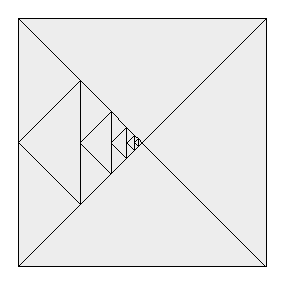
\includegraphics[width=0.24\textwidth]{img/mesh-free}
\caption{Meshes obtained with $k$-irregularity rules, $k = 1,2,3,\infty$.}
\label{fig:academic2}
\end{figure}

Notice that, since $T_n \subset K_1$, all refinements within the elements
$K_2, K_3, K_4$ are forced and they do not improve the resolution. The reader 
can see that the amount of forced refinements decreases as $k$ grows, 
vanishing completely with $k = \infty$.

Next let us choose, e.g., $p=3$, and run the same adaptive procedure for
$n = 1, 2, \ldots, 15$. Figure \ref{fig:academic3a} shows the number of degrees
of freedom corresponding to the final meshes. The horizontal axis represents
the spatial scale $2^{-n}$. 
For the same computations, Figure \ref{fig:academic3b}
shows the condition number of the corresponding stiffness matrices.

\begin{figure}[h!]
\centering
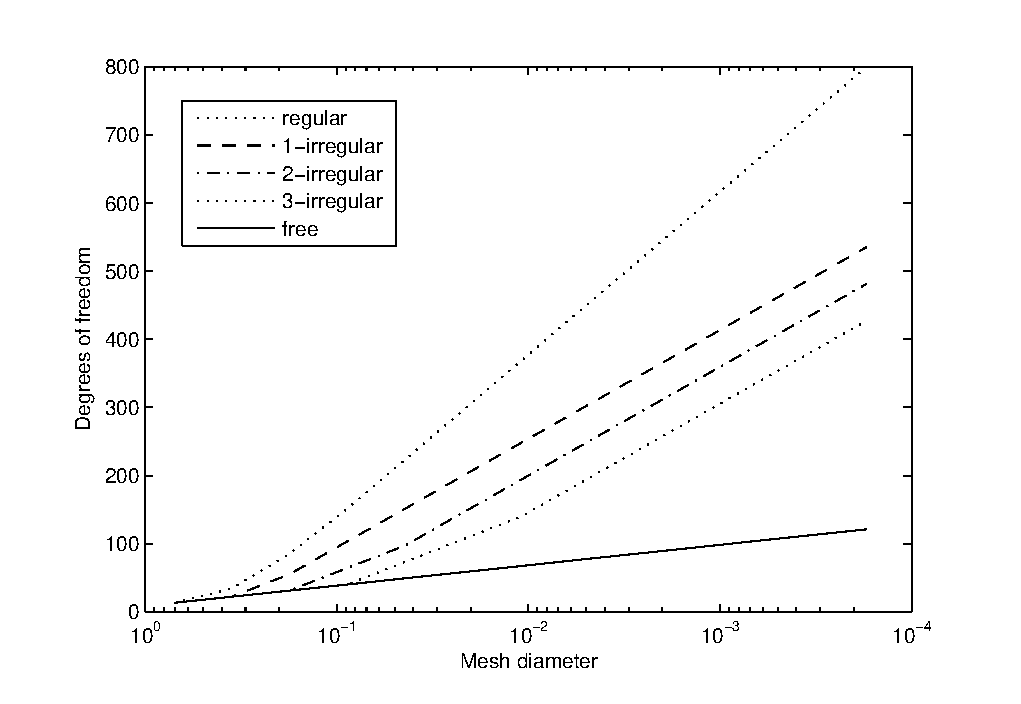
\includegraphics[width=0.9\textwidth]{img/dof-cubic}
\vspace{-4mm}
\caption{Size of the stiffness matrix for final meshes. Level of hanging
         nodes: $k = 0,1,2,3,\infty$.}
\label{fig:academic3a}
\end{figure}
\begin{figure}[h!]
\centering
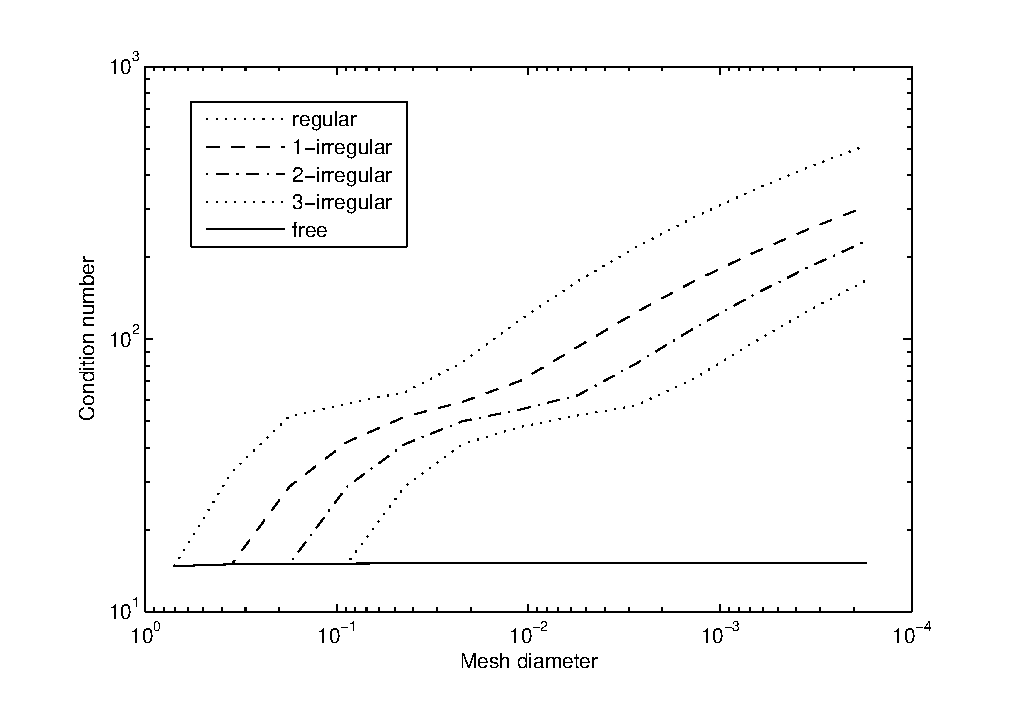
\includegraphics[width=0.9\textwidth]{img/cond-cubic}
\vspace{-4mm}
\caption{Condition number of the stiffness matrix for final meshes.
         Level of hanging nodes: $k = 0,1,2,3,\infty$.}
\label{fig:academic3b}
\end{figure}

In DGFEM, the requirement from the conforming FEM of continuity across mesh edges is dropped, and this means that we only have to be able to calculate fluxes $\bs{f}$ across mesh edges properly (as opposed to conforming finite elements, where we have to take care of the continuity requirement in vertices and on edges). With arbitrary-level hanging nodes, the flux calculation also poses a challenge, and the algorithmic treatment will be described in the section~\ref{sec:data_structures}.

\section{Data structures for $hp$-adaptivity}
\label{sec:data_structures}
The need for mesh adaptivity brings further demands that must be
taken into account in the design of the data structures. A tree-like
hierarchy of element refinement levels must be introduced and also
more complicated neighbor search algorithms are required to correctly
initialize the edge and vertex nodes and the integration points on the edges. The complexity of the data
structures reflects strongly on the complexity of the rest of the
finite element code. 

Simplifying assumptions, such as the
$k$-irregularity rules, are often imposed on the mesh with the aim of reducing code complexity.
However, these assumptions can deteriorate the numerical performance of the code.

In the following we present an original design of data structures for
adaptive meshes, free of any regularity assumptions yet retainign
extreme simplicity.

Calculation of fluxes in DGFEM with arbitrary-level hanging will also be described.

\subsection{Node and element structures}

It should be noted first that we have departed from traditional mesh
data structures storing complete information about the finite element
problem. Our mesh structures contain geometrical information only. The remaining data, including basis function indices, boundary conditions,
polynomial degrees, etc., are stored in separate structures describing
concrete finite element spaces ($H^1$, \Hcurl, ...) and are accessible
via the identification numbers of nodes and elements. This was done to allow
multiple spaces and multiple element types to co-exist on the same mesh,
which is vital for solving multi-physics and coupled problems. See~\cite{my presentation somewhere on my web or what not}

The entire mesh is defined by two arrays of the following C structures.
The first one stores all nodes:
\begin{lstlisting}
  structure Node
  {
    // Type of the Node - either vertex, or edge.
    type;

    // Identificator of the particular Node.
    int id;

    // Physical coordinates of this Node, in case it is a vertex Node.
    coordinate x;
	 coordinate y;

    // Two neighboring elements of this Node, in case it is an edge Node.
	 Element elements[2];
  };
\end{lstlisting}

This structure defines both vertex and edge nodes by utilizig the 
construct to distinguish between an edge and a vertex node. The standard vertex positions {\tt x}, {\tt y},
while typically stored separately, were placed in the vertex variant
of the {\tt Node} structure for simplicity. 
The edge variant contains pointers to the two elements
sharing the edge node (useful eg. when looking for a neighbor of an element sharing a particular edge in order to calculate the numerical flux across the edge).

The member {\tt type} determines the variant of the 
structure. The remaining members are omitted for simplicity.

Elements are defined by the second structure:

\begin{lstlisting}
  struct Element
  {
    // Type of the Element - either triangle, or quadrilateral.
    type;

    // Identificator of the particular Element.
    int id;

	 // Info whether this element is active (has not been refined further).
    boolean active;

    // vertex nodes
    Node vn[4];

    // edge nodes
    Node en[4];
  };
\end{lstlisting}

An element can be either active or inactive, hence the one-bit variable
{\tt active}. Active elements store pointers to the appropriate vertex
and edge nodes. Inactive elements are those which have been split and
are excluded from the computation. Their purpose is to hold pointers
to the descendant elements.

Triangular and quadrilateral elements share the same structure and are
distinguished by the member {\tt type}. The rest of the variables are analogous
to the {\tt Node} structure.

\subsection{Eliminating neighbor search by hashing}
\label{sec:hash}

To properly initialize edge node pointers after reading a mesh file,
one has to construct neighbor lists for all elements and use them in
such a way that only one node is created for each edge. Further
problems arise when certain elements are refined after automatic mesh
adaptation. Unless hanging nodes are removed by extra refinements, no
longer is each edge shared by at most two elements (there can be more of them). Standard neighbor
lists fail to fully capture such situations and thus more complex
data structures, eg. trees \cite{demk1}, have to be introduced.

Loosely inspired by \cite{skala}, we have avoided all of these problems
by introducing a function which, given the {\tt id} numbers of two nodes,
returns a pointer to the node halfway between them. If no such node
exists, it is created first. The task of translating two numbers to
a node pointer is accomplished using a hash table.

We are maintaining two independent layers of nodes: the first layer
contains all vertex nodes, the second all edge nodes. The following
two functions can be called:

\begin{lstlisting}
  Node* get_vertex_node(int id1, int id2);
  Node* get_edge_node(int id1, int id2);
\end{lstlisting}

All nodes, apart from being accessible by their {\tt id} number, can be reached using these functions by
passing the {\tt id}s of their ``parent'' nodes. Top-level vertex nodes (those loaded from the mesh file)
are stored at the beginning of the node array and can be accessed directly without hashing. Mesh
initialization then becomes trivial:

\begin{lstlisting}
  for all Elements
    vertex_numbers = read element vertex id numbers
    for all edges of the Element
      Element.vn = vertex_numbers
      Element.en[0] = get_edge_node(vertex_numbers[0], vertex_numbers[1]);
      Element.en[1] = get_edge_node(vertex_numbers[1], vertex_numbers[2]);
      Element.en[2] = get_edge_node(vertex_numbers[2], vertex_numbers[3]);
      // In case of triangles
      Element.en[3] = get_edge_node(vertex_numbers[3], vertex_numbers[0]);
    }
  }
\end{lstlisting}

Element refinement is also very straightforward. No care must be taken of the neighboring
elements, regardless of their refinement level or even existence:

\begin{lstlisting}
  create_triangle(Node v0, Node v1, Node v2)
  {
    Element e;
    e.vn[0] = v0;
    e.vn[1] = v1;
    e.vn[2] = v2;
    e.en[0] = get_edge_node(v0.id, v1.id);
    e.en[1] = get_edge_node(v1.id, v2.id);
    e.en[2] = get_edge_node(v2.id, v0.id);
  }
  
  void refine_triangle(Element e)
  {
    Node x0 = get_vertex_node(e.vn[0].id, e.vn[1].id);
    Node x1 = get_vertex_node(e.vn[1].id, e.vn[2].id);
    Node x2 = get_vertex_node(e.vn[2].id, e.vn[0].id);
    e.sons[0] = create_triangle(e.vn[0], x0, x2);
    e.sons[1] = create_triangle(x0, e.vn[1], x1);
    e.sons[2] = create_triangle(x2, x1, e.vn[2]);
    e.sons[3] = create_triangle(x0, x1, x2);
    e.active = 0;
  }

  create_quad(Node v0, Node v1, Node v2)
  {
    Element e;
    e.vn[0] = v0;
    e.vn[1] = v1;
    e.vn[2] = v2;
    e.vn[3] = v3;

    e.en[0] = get_edge_node(v0.id, v1.id);
    e.en[1] = get_edge_node(v1.id, v2.id);
    e.en[2] = get_edge_node(v2.id, v3.id);
    e.en[3] = get_edge_node(v3.id, v0.id);
  }
  
  void refine_quad(Element e)
  {
    Node x0 = get_vertex_node(e.vn[0].id, e.vn[1].id);
    Node x1 = get_vertex_node(e.vn[1].id, e.vn[2].id);
    Node x2 = get_vertex_node(e.vn[2].id, e.vn[3].id);
    Node x3 = get_vertex_node(e.vn[3].id, e.vn[0].id);
    e.sons[0] = create_quad(e.vn[0], x0, mid, x3);
    e.sons[1] = create_quad(x0, e.vn[1], x1, mid);
    e.sons[2] = create_quad(mid, x1, e.vn[2], x2);
    e.sons[3] = create_quad(x3, mid, x2, e.vn[3]);
    e.active = 0;
  }
\end{lstlisting}

Each hash table is implemented as an array of linked lists. 
This hash table organization has the advantage of simple node
removal, which is required if a node is no longer needed by any element.

\subsection{Finding all neighbors of an element}
In element-wise assembling procedure with arbitrary-level hanging nodes, when calculating fluxes across mesh edges, one needs values from both sides of the edge. To achieve this, the integration points need to be matched correctly, and proper values in these points from the adjacent element need to be extracted for all involved functions defined on the mesh (basis functions, previous time level solutions). This is not easy to manage. A simplified version of the algorithm is in Appendix 1.

\subsection{Determining node type}

Figure \ref{fig_nodes} shows a simple mesh with hanging nodes. 
Five types of nodes can be identified: standard vertex nodes (A), 
standard edge nodes (B), constrained vertex nodes (C), constrained
edge nodes (D) and finally standard edge nodes and constrained
vertex nodes at the same place (E).

\begin{figure}[H]
  \centering
  \includegraphics[width=0.55\textwidth]{img/nodes.pdf}
  \caption{Mesh with hanging nodes}
  \label{fig_nodes}
\end{figure}

As the elements in the mesh get refined (or derefined), some
nodes are created, others are removed and some change their types.
One has to be able to quickly recognize whether a node is constrained
or unconstrained without searching in the element hierarchy.
This is achieved through the member {\tt ref} of the structure {\tt Node}.
At all times this variable holds the number of elements pointing
to the node. This is the reason why all nodes of an element must be 
\emph{referenced} ({\tt ref} increased) when creating the element and
\emph{un-referenced} ({\tt ref} decreased) when the element is being
refined or deleted, as shown in subsection \ref{sec:hash}.

Now the cases (A) and (C) can be distinguished just by looking at {\tt ref}.
If {\tt ref} = 3, the vertex node is constrained, if {\tt ref} $>$ 3 it
is not constrained. Top-level vertex nodes have {\tt ref} artificially
increased to a large number, which ensures that they are always treated as
unconstrained. Similarly, if {\tt ref} = 1 for an edge node, it is
constrained (D); if {\tt ref} = 2 it is unconstrained (D).

The case (E) can be detected by calling the function
{\tt peek\_*\_node}, which works the same way as
{\tt get\_*\_node}, with the exception that the node is not 
created if it does not exist. 

A node is deleted any time its {\tt ref} reaches zero.

\section{Automatic $hp$-adaptivity}

The major difference between adaptivity in standard FEM and adaptivity
in $hp$-FEM is the large number of element refinement options in the
latter case. In standard $h$-adaptivity, elements can only be subdivided in space,
e.g., using the {\em red-green} refinement technique (see \cite{aksoylu} and the
references therein). In $hp$-adaptivity, one can either increase the polynomial
degree of elements without subdividing them in space or one can split elements
in space and distribute the polynomial degree on the subelements in multiple ways.

\subsection{Reference solution}

The presence of many $hp$-refinement options per element implies that
classical error estimates (in the form of one number per element)
do not provide enough information to guide $hp$-adaptivity. Instead,
one needs to use some information about the {\em shape} of
the error function $e_{h,p} = u - u_{h,p}$. In principle, this information
could be obtained by estimating higher derivatives, but such approach
is not very practical. Usually it is more convenient to use
a {\em reference solution}, i.e., an approximation $u_{ref}$ which is
at least one order more accurate than the coarse mesh solution $u_{h,p}$.
The $hp$-adaptivity is then guided by an a-posteriori error estimate
of the form
\be\label{errest}
e_{h,p} = u_{ref} - u_{h,p}
\ee

Such approach, as opposed to classical error estimates, is virtually
equation-independent. In this work we are constructing the enriched
finite element space by uniform subdivision of all mesh elements and 
by increasing all element polynomial degrees by one, i.e.
\bd
  u_{ref} = u_{h/2,p+1}
\ed

The reference solution $u_{ref}$ can be obtained efficiently by
utilizing information about lower frequencies from $u_{h,p}$
\cite{demk1,SoDe,solin1} if iterative solvers are used or by 
reconstructing the LU decomposition of the stiffness matrix
from the LU-decomposed coarse mesh stiffness matrix when using
direct sparse solvers, e.g. UMFPACK. However, we have not
attempted any such optimization in this work, even though we
admit that this issue must be addressed in order for the methods
to be usable in practice.


\subsection{Outline of the algorithm}

The outer loop of our adaptivity algorithm is formally similar
to the one of L.~Demkowicz et al. (see \cite{derade}), with minor
differences. The outline of the algorithm is as follows:
\begin{enumerate}
\item Assume an initial coarse mesh $\Tau_{h,p}$ consisting of piecewise-constant, linear or
      quadratic elements. User input includes
      \begin{enumerate}
			\item prescribed relative tolerance $TOL > 0$ for the
			      rate of energy norm of the approximate error function (\ref{errest}) and energy norm of the approximate solution 
			\item threshold ERRT specifying how many elements should be refined in each $hp$-adaptivity step
		\end{enumerate}
\item User input may also include
		\begin{enumerate}
			\item maximum increase of degrees of freedom $MAX\_STEP\_NDOF$ in each adaptivity step\\OR\\
			\item maximum number of degrees of freedom $MAX\_NDOF$
      \end{enumerate}

\item Create a fine mesh, $\Tau_{h/2,p+1}$

\item Compute fine mesh approximation $u_{h/2,p+1} \in V_{h/2,p+1}$ on $\Tau_{h/2,p+1}$.

\item Project the fine mesh approximation onto the coarse mesh $\Tau_{h,p}$. In this way, obtain a coarse mesh approximation.

\item Calculate the desired norm ($H^1$ norm, $H^1$ seminorm, $L^2$ norm, custom norm) of the fine mesh approximations $NORM_i$ on every element $K_i$ in the mesh, $i = 1, 2, \ldots, M$. Construct the approximate error function (\ref{errest}) as the difference between the fine and coarse mesh approximations, calculate its energy norm $ERR_i$ on every element $K_i$ in the mesh, $i = 1, 2, \ldots, M$. Calculate the global error estimate $$ERR = \lo\sum_{i=1}^M ERR_i\ro / \lo\sum_{i=1}^M NORM_i\ro.$$
      
\item If $ERR \le TOL$, stop computation and proceed to postprocessing.

\item Sort all elements into a list $L$ according to their value $ERR_i / NORM_i$
      in decreasing order.
      
\item Determine the maximum of element errors, $ERR_{max} = \max\{ERR_i / NORM_i\}$,
      by taking the first item of L.
      
\item Let {\it NDOF} be the current number of degrees of freedom of $\Tau_{h,p}$. Repeat the following cycle:
      \begin{enumerate}
			\item If $MAX\_STEP\_NDOF$ is set, and if the already added degrees of freedom in this $hp$-adaptivity step is greater than $MAX\_STEP\_NDOF$, break the cycle
      	\item Take the next element $K_i$ from the list $L$
      	\item If $ERR_i / NORM_i < ERRT \cdot ERR_{max}$, break the cycle
      	\item Perform $hp$-refinement of $K_i$ (to be described in more detail below).
      	\item If $MAX\_NDOF$ is set, and if the total number of degrees of freedom is now greater than $MAX\_NDOF$, break
      	the cycle
      \end{enumerate}
      
\item Continue with step C.\\
\end{enumerate}

The crucial issue in the outer loop is determining how many elements should be refined.
In \cite{derade} all elements whose error $ERR$ is greater than 70\% of the maximum
error $ERR_{max}$ are taken (ie. $ERRT = 0.7$). This is a relatively conservative
choice which leads to good convergence curves, but may result in too many steps
of the algorithm, which should be avoided as the evaluation of $u_{ref}$ is very
expensive. Our experience shows that setting $ERRT$ as low as 15\% results
in equally good convergence curves for most problems, but achieved in much fewer
steps and in turn in much shorter time. Occasionally, however, the low value of
$ERRT$ may cause too many elements to be refined and thus we introduced the 
limit $MAX\_STEP\_NDOF$ of the number of degrees of freedom added in each step. Typically,
one should not increase the number of degrees of freedom in each step by a large number.

\subsection{Selecting optimal $hp$-refinement}

The algorithm for determining optimal $hp$-refinements in \cite{derade} is 
quite complex. Built upon the projection-based interpolation theory,
it first finds optimal $hp$-refinement of mesh edges using a 1D
version of the $hp$-adaptive algorithm. The edge refinements then
determine $h$-refinement of elements. Finally, best polynomial
degrees for element interiors are selected. Each step of the algorithm
represents a considerable implementation burden.

We have implemented a much simpler scheme, which is local in the sense
that element refinements are selected without regard to the refinements
of neighboring elements. For all elements $K\in \Tau_{h,p}$ of polynomial
degree $p$ picked by the outer loop we consider the following 
$N = 83$ $hp$-refinement options:
\begin{enumerate}
\item Increase the polynomial degree of $K$ to $p+1$ without spatial subdivision.
\item Increase the polynomial degree of $K$ to $p+2$ without spatial subdivision.
\item Split $K$ into four similar triangles $K_1, K_2, K_3, K_4$.
      Define $p_0$ to be the integer part of $(p+1)/2$.
      For each $K_i$, $1 \le i \le 4$ consider polynomial
      degrees $p_0 \le p_i \le p_0 + 2$.
\end{enumerate}
For each of these $N$ options we perform a standard e.g. $L_2$-projection
of the reference solution $u_{ref}$ onto the corresponding polynomial
space. The candidate with smallest projection error is selected
for $hp$-refinement of the element $K$.

Each of the $N$ projection problems requires the solution of a small
system of linear algebraic equations with a symmetric positive-definite
matrix. The solution of these systems can be further optimized by exploiting
the incremental nature of the Cholesky decomposition algorithm 
and the fact that the spaces in item 3 above are partially embedded.
\paragraph{Example}
We again solve the model problem~\eqref{ade} with the same settings as in Paragraph~\ref{par:model_example}. This time, automatic hp-adaptivity will be used. Although the maximum value of the exact solution is $1.0$, due to the presence of undershoots and overshoots, the maximum values here are higher, as was seen already in section~\ref{sec:DG}. This can be avoided by using a suitable shock capturing method, as it is done in the last chapter with numerical examples for the Euler equations.
\begin{figure}[H]
\begin{center}
\includegraphics[width=0.48\textwidth]{minor_examples/Sln1.png}\ \ \ 
\includegraphics[width=0.48\textwidth]{minor_examples/Space1.png}
\end{center}
\vspace{-4mm}
\caption{Solution and a mesh, relative error between the fine mesh and the coarse mesh approximation: 25.7746\%.}
\end{figure}

\begin{figure}[H]
\begin{center}
\includegraphics[width=0.48\textwidth]{minor_examples/Sln2.png}\ \ \ 
\includegraphics[width=0.48\textwidth]{minor_examples/Space2.png}
\end{center}
\vspace{-4mm}
\caption{Solution and a mesh, relative error between the fine mesh and the coarse mesh approximation: 10.3565\%.}
\end{figure}

\begin{figure}[H]
\begin{center}
\includegraphics[width=0.48\textwidth]{minor_examples/Sln3.png}\ \ \ 
\includegraphics[width=0.48\textwidth]{minor_examples/Space3.png}
\end{center}
\vspace{-4mm}
\caption{Solution and a mesh, relative error between the fine mesh and the coarse mesh approximation: 5.58551\%.}
\end{figure}

\begin{figure}[H]
\begin{center}
\includegraphics[width=0.48\textwidth]{minor_examples/Sln5.png}\ \ \ 
\includegraphics[width=0.48\textwidth]{minor_examples/Space5.png}
\end{center}
\vspace{-4mm}
\caption{Solution and a mesh, relative error between the fine mesh and the coarse mesh approximation: 2.43584\%.}
\end{figure}

\begin{figure}[H]
\begin{center}
\includegraphics[width=0.48\textwidth]{minor_examples/Sln7.png}\ \ \ 
\includegraphics[width=0.48\textwidth]{minor_examples/Space7.png}
\end{center}
\vspace{-4mm}
\caption{Solution and a mesh, relative error between the fine mesh and the coarse mesh approximation: 1.27544\%.}
\end{figure}

\begin{figure}[H]
\begin{center}
\includegraphics[width=0.48\textwidth]{minor_examples/Sln9.png}\ \ \ 
\includegraphics[width=0.48\textwidth]{minor_examples/Space9.png}
\end{center}
\vspace{-4mm}
\caption{Solution and a mesh, relative error between the fine mesh and the coarse mesh approximation: 0.919277\%.}
\end{figure}

\subsection{Automatic $hp$-adaptivity for time-dependent problems}

In the previous chapters we were concerned with the stationary problems. Let us now discuss automatic adaptivity for transient problems. Time-dependent coupled problems are challenging since one has to capture transient phenomena with sufficient accuracy, while the size of the problem must stay reasonably small. This leads to an obvious need for dynamically changing meshes for such problems. In most scientific computations, where dynamical meshes are used for time-dependent problems, data-transfer methods are necessary to move solution values between meshes for different time levels. As shown in subsection \ref{sec:data-transfer}, data-transfer methods cause additional error and in case of time-dependent problems repeated transfers (usually simple interpolation) between meshes can have disastrous consequences.

We use orthogonal projections of the solution of transient problems using dynamical $hp$-meshes obtained fully automatically by the $hp$-adaptive algorithm. With the automatic $hp$-adaptivity and dynamical meshes the question of coarsening meshes between time levels arises. Mesh derefinement is particularly important in problems where sharp fronts (internal layers) move through the domain leaving smooth solutions behind them. We propose an original coarsening algorithm suitable for $hp$-FEM based on the \textit{super-coarse solution}, which results in substantially fewer adaptive iterations.

The adaptive $hp$-FEM algorithm for time-dependent problems we use is obtained by combining the classical Rothe's method for time discretization with adaptive $hp$-FEM for the space discretization.
The Rothe's method is a natural counterpart of the widely used Method of Lines (MOL). 
Recall that the MOL performs discretization in space while keeping the time variable continuous, which leads to a system of ODEs in time. The Rothe's method, on the contrary, preserves the continuity of the spatial variable while discretizing time. In every time step, an evolutionary PDE is approximated by means of one or more time-independent ones. For one step methods (such as implicit Runge-Kutta), the number of the time-independent equations per time step is proportional to the order of accuracy of the time discretization method. For example, when employing the implicit Euler method, one has to solve just one time-independent PDE per time step:

\begin{equation}\label{rothe}
 \frac{\partial u}{\partial t} = F(t, u) \quad \Rightarrow \quad \frac{u^{n+1} - u^n}{\Delta t} = F(t^{n+1}, u^{n+1})
\end{equation}

The Rothe's method is fully equivalent to the MOL if no adaptivity in space or time takes place, but it provides a better setting for the application of spatially adaptive algorithms. The spatial discretization error can be controlled by solving the time-independent equations adaptively, and the size of 
the time step can be adjusted using standard ODE techniques \cite{deuflhard,hairer1,hairer2}.

In this subsection, first the notion of \emph{dynamical meshes} will be presented, then the refining and coarsening algorithms for time dependent problems are shown.

\paragraph{Dynamical meshes}

By ${\cal T}_m$ let us denote a uniform coarse mesh covering the computational domain 
$\Omega$. This mesh (called {\em master mesh}) is shared by the solution at all time levels, in other words all meshes can be obtained from this mesh by elementary refinements. At each time instant $t_n$ an optimal mesh is found to suit the best the solution $\bfu^n(\bfx)$. On the $(n+1)$st time level, the approximated solution $\bfu^n(\bfx)$, that has been obtained in the previous time step, is used as data. Note, however, that $\bfu^n$ is defined on a locally refined mesh that was created automatically during the $n$th time step, while the unknown $\bfu^{n+1}$ is solved adaptively starting from a coarser mesh. As a result, the meshes obtained on each time level are different, i.e., the mesh changes dynamically in time. 

As mentioned above, in transient problems the optimal meshes are on each time level obtained automatically and they can change from one time step to another, which induces need for both refining and coarsening strategies.

\subsubsection{Refining algorithm}

In Chapter \ref{ch:adapt} the goal of adaptive algorithm was to decrease the error as low as possible. On the other hand for time-dependent problems we want to sustain the space error on approximately the same level, which would result into meshes with smoothly changing number of degrees of freedom. For time-dependent problems, as well as for time-independent, the amount of elements refined in one adaptive iteration will depend on the global solution error estimate in that iteration. As described, one can drive the refining algorithm by variables $TOL$, $ERRT$, $MAX\_STEP\_NDOF$, $MAX\_NDOF$.

\subsubsection{Coarsening algorithm}

The most primitive strategy to coarsen the mesh on the next time level is to start on each level from the very coarse (master) mesh and perform the automatic adaptivity to find the optimal mesh for a particular solution $\bfu^n(\bfx)$. Although this would result in the most optimal meshes in each iteration, it is virtually impossible to carry it out due to the immense computational time demands. Moreover, a lot of work would be wasted since the solutions from two adjacent time steps usually differ only mildly even though the solution changes significantly in the whole time domain. Global derefinement would result in similar difficulties. 

We present a coarsening algorithm that prepares the mesh for the adaptive algorithm on the next time level by local derefinements. Thus, we remove only unnecessary refinements from previous time levels. In this way the meshes for particular time steps are suboptimal, but the number of adaptive iterations performed in each time step significantly decreases.

In higher-order finite element method we have two questions. First question is which elements can be coarsened and second is how to coarsen them. In $hp$-FEM we can either decrease the polynomial order of the element or derefine the element geometrically. We can also employ various choices for assigned polynomial order. Situation is depicted in Fig. \ref{fig:coarse}. 

\begin{figure}[ht]
  \centering
  \includegraphics[width=0.7\textwidth]{img/coarsening.pdf}
  \caption{Coarsening choices for an element.}
  \label{fig:coarse}
\end{figure}

However, the coarsening serves only to prepare the mesh for the next adaptive process, thus we do not have to search for the best unrefinement as we do in case of refinements. It is perfectly sufficient to perform any coarsening that does not cause error increase and the mesh will optimize itself in the next adaptive loop.
So far, to keep the algorithm reasonably simple we allow only coarsening as reversing of previous element refinements. In this way the tree-like structure of meshes starting from the {\em master mesh} is preserved. Unfortunately, the coarsening algorithm cannot be just an opposite to the refining. While with the refining algorithm we are seeking for the best candidate in the sense of error decrease, here we are looking for a candidate whose error will not exceed some tolerance (so that it would not be subsequently refined).

Let us denote by $e_{max}$ the error of the element with maximal error from the last adaptive iteration. From Alg. \ref{alg:adapt} from Chapter \ref{ch:adapt} we know that errors of all elements are below $ERR_{max}$ and that it should be satisfied as well after the coarsening procedure. First we calculate so called {\em super-coarse solution} for polynomial orders. By that we mean that polynomial order on all elements is decreased by one. We calculate error estimates for all elements in the super-coarse mesh with respect to the reference solution and lower the polynomial order on those elements whose error after coarsening is less than $k * ERR_{max}$, where parameter $k\in(0,1)$ is chosen to ensure that element will not be subsequently refined in the adaptive procedure on the next time level. Similar procedure is run for a spatial coarsening -- {\em super-coarse solution} is calculated on the mesh where all elements with four active subelements are coarsened and polynomial order on such elements is assigned to be the maximum of orders on four subelements. In a similar way as before we determine which elements can be also spatially unrefined without significant increase of the error.

The whole procedure for time-dependent problems with the refining and coarsening strategy is described in Alg. \ref{alg:dynamic}. Effectivity of the approach is demonstrated on the numerical examples in the last chapter of this thesis.

\begin{algorithm}[!ht]
  \caption{Adaptive algorithm for time-dependent problems with improved stopping criterion.}
\label{alg:dynamic}
  \SetAlgoLined
  \ForEach{time level}{
    \Repeat{not done}{
       compute reference solution $u_{ref}$\;
       project to get a solution on current mesh $u$\;
       evaluate global error estimate $ERR_{gl}$ and local errors on elements $ERR_i$\;
       \eIf{$ERR_{gl} < TOL$}{
          done = true\;
          break\;
          }{
          sort all elements by their error\;
          processed error = 0\;
         \ForEach{element}{
         \eIf{(processed error $> c * (ERR_{gl}$ - TOL)) \textbf{or} ($ERR_i < k * ERR_{max}$)}{
           done = true\;
           break\;
         }{
           find optimal refinement\;
           processed error $+= ERR_i$\;
         }
         }
       }
    }
    calculate super-coarse solution for polynomial orders\;
    decrease polynomial orders when possible\;
    calculate super-coarse solution for spatial refinements\;
    geometrically coarsen elements when possible\;
  }
\end{algorithm}


\chapter{Dicontinuous Galerkin discretization of the Euler equations}
 For what follows, we introduce the following notation. By $\varphi|_{\Gamma_{ij}}$ and $\varphi|_{\Gamma_{ji}}$ we denote the values of $\varphi$ on $\Gamma_{ij}$ considered from the interior and the exterior of $K_i$ respectively. The symbols
  \be
  \left<\varphi\right>_{ij} = \frac12\lo\varphi|_{\Gamma_{ij}} + \varphi|_{\Gamma_{ij}}\ro,\ \ \left[\varphi\right]_{ij} = \varphi|_{\Gamma_{ij}} - \varphi|_{\Gamma_{ji}}
  \ee
  stand for the average of the two values $\varphi|_{\Gamma_{ij}}$ and $\varphi|_{\Gamma_{ji}}$, and their difference (i.e. jump of $\varphi$ on $\Gamma_{ij}$) respectively.
\section{Numerical Fluxes}
  The DGFEM discretization of the Euler equations in their conservative form follows the principles of the section~\ref{sec:DG}. We take the equations in the form~\eqref{conservative_form}. We leave the time derivative for now, and we need to find suitable numerical fluxes to approximate the fluxes $\partial{\bs{f}}_x, \partial{\bs{f}}_y$ through the faces $\Gamma_{ij}$. The numerical fluxes will be sought so that the requirements from the subsection~\ref{subsec:numflux_properties} are met.
\paragraph{Construction of some numerical fluxes}
The following type of numerical fluxes are usually called \emph{flux vector splitting schemes} and we use the knowledge from the section~\ref{sec:euler_properties}, namely~\eqref{P_definition},~\eqref{first_homo}, ..., and~\eqref{final_p_diag}. On the basis of~\eqref{final_p_diag} we define the matrices
\be
\Lambda^{\pm} = \text{diag}\lo\lambda_1^{\pm}, ..., \lambda_m^{\pm}\ro,\ \ |\Lambda| = \text{diag}\lo|\lambda_1|, ..., |\lambda_m|\ro.
\ee
Also we define
\be
\mathbb{P}^{\pm} = \mathbb{P} \Lambda^{\pm} \mathbb{P}^{-1},\ \ |\mathbb{P}| = \mathbb{P} |\Lambda| \mathbb{P}^{-1}.
\ee
These matrices depend on $\bs{w}\in D$ and $\bs{n}\in\mc{S}_1$. Now we define the following two schemes that will later be used in the numerical examples.
\begin{enumerate}
\item \emph{The Steger-Warming scheme} has the numerical flux:
$$ \bs{H}_{SW}\lo\bs{u},\bs{v},\bs{n}\ro = \mathbb{P}^+\lo\bs{u},\bs{n}\ro\bs{u} + \mathbb{P}^-\lo\bs{v},\bs{n}\ro\bs{v},\ \ \bs{u},\bs{v}\in D,\ \bs{n}\in\mc{S}_1.$$
This scheme is rather diffusive, so another scheme is preferred.
\item  \emph{The Vijayasundaram scheme} has the numerical flux:
$$ \bs{H}_{V}\lo\bs{u},\bs{v},\bs{n}\ro = \mathbb{P}^+\lo\frac{\bs{u} + \bs{v}}{2},\bs{n}\ro\bs{u} + \mathbb{P}^-\lo\frac{\bs{u} + \bs{v}}{2},\bs{n}\ro\bs{v},\ \ \bs{u},\bs{v}\in D,\ \bs{n}\in\mc{S}_1.$$
\end{enumerate}

This scheme contains a \emph{partial upwinding}, where the flux is computed at the point $x_{i + \frac{1}{2}}\ \lo x_{i - \frac{1}{2}}\ro$ with the use of the value $\bs{w}_i^k$ or $\bs{w}_{i+1}^k \lo \bs{w}_{i-1}^k \text{ or } \bs{w}_i^k\ro$ corresponding to the mesh point located in the upwind direction wrt. the propagation speed given by the eigenvalues $\lambda_i$. In the Steger-Warming scheme we speak of a \emph{full upwinding}.
\paragraph{}
Another possible construction of the numerical flux is based on the rotational invariance of the Euler equations, see Section~\ref{sec:rot_inv}. We introduce a new Cartesian coordinate szstem $\tilde{x}_1, ..., \tilde{x}_N$ with the origin at the midpoint of the face $\Gamma$, the coordinate $\tilde{x}_1$ oriented in the direction of the normal $\bs{n}$ and $\tilde{x}_2, ..., \tilde{x}_N$ tangent to $\Gamma$. The rotational invariance of the Euler equations implies that these equations have the form
\be
\frac{\partial\bs{q}}{\partial t} + \sum_{s = 1}^2\frac{\partial\bs{f}_s\lo\bs{q}\ro}{\partial\tilde{x}_s} = 0,
\ee
where
$$
\bs{q} = \mathbb{Q}\lo\bs{n}\ro\bs{w}
$$
with matrix $\mathbb{Q}\lo\bs{n}\ro$ defined in~\eqref{Q}. The tangential derivatives are neglected, and only the system with one space variable is considered:
\be
\label{one_variable_system}
\frac{\partial\bs{q}}{\partial t} + \frac{\partial\bs{f}_1\lo\bs{q}\ro}{\partial\tilde{x}_1} = 0.
\ee
Then the numerical flux is defined in the form
\be
\bf{H}\lo\bs{u}, \bs{v}, \bs{n}\ro = \mathbb{Q}^{-1}\lo\bs{n}\ro\bs{g}_R\lo\mathbb{Q}\lo\bs{n}\ro\bs{u},\mathbb{Q}\lo\bs{n}\ro\bs{v}\ro,
\ee
where $\bs{g}_R = \bs{g}_R\lo\bs{q}_1, \bs{q}_2\ro$ is a numerical flux (so-called \emph{approximate Riemann solver}, see~\cite{feistauer}) for the system~\eqref{one_variable_system} with one space variable.
This numerical flux is complicated to be linearized, and because we wanted to employ a semi-implicit method for time integration, we opted for the Vijayasundaram numerical flux in most cases.

\section{Time discretization}
This section closely follows~\cite{DF04}. Using numerical fluxes we can introduce new forms
\begin{eqnarray}
\nonumber
\lo\bs{w}_h,\boldsymbol{\varphi}_h\ro & = & \int_{\Omega}\bs{w}_h\lo\bs{x}\ro\cdot\boldsymbol{\varphi}_h\lo\bs{x}\ro d\bs{x},\\
\label{tilde_b}
\tilde{b}_h\lo\bs{w}_h,\boldsymbol{\varphi}_h\ro & = &-\sum_{K\in\mc{T}_h}\int_K\sum_{s=1}^2\bs{f}_s\lo\bs{w}_h\lo\bs{x}\ro\ro\cdot\frac{\partial\boldsymbol{\varphi}_h\lo\bs{x}\ro}{\partial x_s} d\bs{x} \\ \nonumber
& + & \sum_{K_i\in\mc{T}_h}\sum_{j\in\mc{S}\lo i\ro} \int_{\Gamma_{ij}}\bs{H}\lo\bs{w}\lo t\ro|_{\Gamma_{ij}}, \bs{w}\lo\bs{x}\ro|_{\Gamma_{ji}},\bs{n}_{ij}\ro\cdot \boldsymbol{\varphi}_h\lo\bs{x}\ro dS
\end{eqnarray}

for $\bs{w}_h, \boldsymbol{\varphi}_h\in \left[V_h\right]^4$. We say that $\bs{w}_h$ is the approximate solution of~\eqref{conservative_form} in $Q_T = \Omega\times\lo 0,T\ro$,
if it satisfies the conditions
\begin{enumerate}
\item \be\bs{w}_h\in\mc{C}^1\lo\left[0,T\right],\left[V_h\right]^4\ro\ee,
\item \be\label{approx_sol} \frac{d}{dt}\lo\bs{w}\lo t\ro,\boldsymbol{\varphi}_h\ro + \tilde{b}_h\lo\bs{w}_h\lo t \ro, \boldsymbol{\varphi}_h\ro = 0\ \ \forall\boldsymbol{\varphi}_h\in\left[V_h\right]^4\forall t\in\lo 0,T\ro\ee,
\item \be\bs{w}_h\lo 0\ro = \Pi_h\bs{w}^0\ee,
\end{enumerate}
where $\Pi_h\bs{w}^0$ is the $L^2$-projeftion of the initial condition $\bs{w}^0$ onto the space $\left[V_h\right]^4$. If we set $p=0$, then we obviously obtain the finite volume method.
\paragraph{}
Relations~\eqref{approx_sol} represent a system of ordinary differential equations which can be solved by a suitable numerical method. Since we are interested in applying the Rothe's method, we now want to discretize the time derivative. In order to do so, we consider a partition $0 = t_0 < t_1 < t_2 < ...$ of the time interval $\lo 0, T\ro$ and set $\tau_k = t_{k+1} - t_k$. We use the notation $\bs{w}_h^k$ for the approximation of $\bs{w}_h\lo t_k\ro$. Then we apply the simple implicit \emph{backward Euler method} and our \emph{discrete problem} reads: for each $k\geq 0$ find $\bs{w}_h^{k+1}$ such that
\begin{enumerate}
\item \be\bs{w}_h^{k+1}\in\left[V_h\right]^4\ee,
\item \be\label{approx_sol_discretized} \lo\frac{\bs{w}_h^{k+1} - w_h^k}{\tau_k},\boldsymbol{\varphi}_h\ro + \tilde{b}_h\lo\bs{w}_h^{k+1}, \boldsymbol{\varphi}_h\ro = 0\ \ \forall\boldsymbol{\varphi}_h\in\left[V_h\right]^4,\ k = 0, 1, ...\ee
\item \be\bs{w}_h^0 = \Pi_h\bs{w}^0\ee.
\end{enumerate}
This scheme leads to a system of highly nonlinear algebraic equations whose numerical solution is rather complicated. In order to simplify the problem, in the following we shall linearize relations~\eqref{approx_sol_discretized} and obtain a linear system.
\subsection{Linearization}
By~\eqref{tilde_b}, for $\bs{w}_h^{k+1},\boldsymbol{\varphi}_h\in\left[V_h\right]^4$ we have
\begin{eqnarray}
\tilde{b}_h\lo\bs{w}_h^{k+1},\boldsymbol{\varphi}_h\ro & = &-\sum_{K\in\mc{T}_h}\int_K\sum_{s=1}^2\bs{f}_s\lo\bs{w}_h^{k+1}\lo\bs{x}\ro\ro\cdot\frac{\partial\boldsymbol{\varphi}\lo\bs{x}\ro}{\partial x_s} d\bs{x} \ \ (=: \tilde{\sigma}_1)\\
+ \sum_{K_i\in\mc{T}_h}\sum_{j\in{S}\lo i\ro} & & \int_{\Gamma_{ij}} \bs{H}\lo\bs{w}_h^{k+1}|_{\Gamma_{ij}}, \bs{w}_h^{k+1}|_{\Gamma_{ji}},\bs{n}_{ij}\ro\cdot \boldsymbol{\varphi}_h\lo\bs{x}\ro dS \ \ (=: \tilde{\sigma}_2)
\end{eqnarray}
The terms $\tilde{\sigma}_1$, and $\tilde{\sigma}_2$ are linearized as follows. We set
\be
\tilde{\sigma}_1\approx\sigma_1 = \sum_{K\in\mc{T}_h}\int_K\sum_{s=1}^2\mathbb{A}_s\lo\bs{w}_h^k\lo\bs{x}\ro\ro\bs{w}_h^{k+1}\lo\bs{x}\ro\cdot\frac{\partial\boldsymbol{\varphi}_h\lo\bs{x}\ro}{\partial x_s}d\bs{x}
\ee
and
\begin{eqnarray}
\tilde{\sigma}_2\approx\sigma_2 = \sum_{K_i\in\mc{T}_h}\sum_{j\in s\lo i \ro}\int_{\Gamma_{ij}}\left[\mc{P}^+\lo \left<\bs{w}_h^k\right>_{ij},\bs{n}_{ij}\ro\bs{w}_h^{k+1}|_{\Gamma_{ij}} \right. \\+ \left. \mc{P}^-\lo \left<\bs{w}_h^k\right>_{ij},\bs{n}_{ij}\ro\bs{w}_h^{k+1}|_{\Gamma_{ji}}\right] \cdot \boldsymbol{\varphi}_h dS \\+ 
\sum_{K_i\in\mc{T}_h}\sum_{j\in{S}\lo i\ro\backslash s\lo i \ro} \int_{\Gamma_{ij}}\bs{H}\lo\bs{w}_h^{k+1}|_{\Gamma_{ij}}, \bs{w}_h^{k+1}|_{\Gamma_{ji}},\bs{n}_{ij}\ro\cdot \boldsymbol{\varphi}_h\lo\bs{x}\ro dS.
\end{eqnarray}
We omit the linearization of the fluxes across domain boundaries, for details see~\cite{DF04}. Finally, we define the form
\be
b_h\lo\bs{w}_h^k,\bs{w}_h^{k+1},\boldsymbol{\varphi}_h\ro = -\sigma_1 + \sigma_2.
\ee
The form is linear wrt. the second and third variable. Using this form we come to the following \emph{semi-implicit linearized numerical scheme}: for each $k\geq 0$ find $\bs{w}_h^{k+1}$ such that
\begin{enumerate}
\item \be\bs{w}_h^{k+1}\in\left[V_h\right]^4\ee,
\item \be\lo\bs{w}_h^{k+1},\boldsymbol{\varphi}_h\ro + \tau_k {b}_h\lo\bs{w}_h^k, \bs{w}_h^{k+1},\boldsymbol{\varphi}_h\ro = \lo\bs{w}_h^k, \boldsymbol{\varphi}_h\ro\ \ \forall\boldsymbol{\varphi}_h\in\left[V_h\right]^4,\ k = 0, 1, ...\ee
\item \be\bs{w}_h^0 = \Pi_h\bs{w}^0\ee.
\end{enumerate}

\section{Boundary conditions}
In all examples in the next chapter, the boundary of the computational domain $\Omega$ is divided into three parts.
\begin{enumerate}
\item On a fixed impermeable wall $\Gamma_W\subset\partial\Omega$ we use the condition $\bs{v}\cdot\bs{n} = 0$. Then the flux $\mc{P}\lo\bs{w},\bs{n}\ro$ has the form
\begin{eqnarray}
\mc{P}\lo\bs{w},\bs{n}\ro & = & \sum_{s=1}^2\bs{f}_s\lo\bs{w}\ro n_s \\ & = & \lo\bs{v}\cdot\bs{n}\ro\bs{w} + p \lo 0, n_1, n_2, \bs{v}\cdot\bs{n}\ro^T \\ & = & p\lo 0, n_1, n_2, 0\ro^T,
\end{eqnarray}
which is uniquely determined on $\Gamma_W$ by the extrapolated value of the pressure, i.e. by $p_j^k := p_i^k$. Therefore, on the part $\Gamma_W$ of the boundary we define the numerical flux
\be
\bs{H}\lo\bs{w}_i^k, \bs{w}_j^k, \bs{n}\ro = p_i^k\lo 0, n1, n2, 0\ro^T.
\ee
We can see that on the impermeable part of the boundary, 2 eigenvalues $\lambda_2, \lambda_3$ are zero, and the eigenvalue $\lambda_1$ is negative, and the eigenvalue $\lambda_4$ is positive. We prescribe only $\bs{v}\cdot\bs{n} = 0$, and extrapolate the pressure.
\item
On the inlet
$$
\Gamma_I\lo t \ro = \left\{x\in\partial\Omega; \bs{v}\lo x, t\ro \cdot \bs{n}\lo x \ro < 0\right\}
$$
and the outlet
$$
\Gamma_O\lo t \ro = \left\{x\in\partial\Omega; \bs{v}\lo x, t\ro \cdot \bs{n}\lo x \ro > 0\right\}
$$
parts of the boundary it is necessary to use nonreflecting boundary conditions. In this case we used the so-called \emph{characteristics-based} bounadry conditions, according to~\cite{sbornik konference HYP06}.
Using the rotational invariance, we tranform the Euler equations to the coordinates $\tilde{x}_1$, in the direction of the outer normal $\bs{n}$ to the boundary, and $\tilde{x}_2$, tangential to the boundary and linearize the resulting system around the state $\bs{q}_{ij} = \mathbb{Q}\lo\bs{n}_{ij}\ro$. Then we obtain the linear system
\be
\frac{\partial\bs{q}}{\partial t} +\mathbb{A}_1\lo\bs{q}_{ij}\ro\frac{\partial\bs{q}}{\partial\tilde{x}_1} = 0,
\ee
for the vector-valued function $\bs{q} = \mathbb{Q}\lo\bs{n}_{ij}\ro\bs{w}$, considered in the set $\lo -\infty,0\ro\times\lo 0,\infty\ro$ and equipped with the initial and boundary conditions
\begin{eqnarray}
\bs{q}\lo\tilde{x}_1,0\ro & = & \bs{q}_{ij},\ \ \tilde{x}_1 < 0,\\
\bs{q}\lo 0,t\ro & = & \bs{q}_{ij},\ \ t > 0.
\end{eqnarray}
The goal is to choose $\bs{q}_{ij}$ in such a way that this initial-boundary value problem is well-posed, i.e. has a unique solutions. The method of characteristics leads to the following process:
\paragraph{}
Let us put $\bs{q}^*_{ji} = \mathbb{Q}\lo\bs{n}_{ij}\ro\bs{w}_{ji}^*$, where $\bs{w}_{ji}$ is a prescribed boundary state at the inlet or outlet. We calculate eigenvectors $\bs{r}_s$ corresponding to the eigenvalues $\lambda_1, ..., \lambda_4$, of the matrix $\mathbb{A}_1\lo\bs{q}_{ij}\ro$, arrange them as columns in the matrix $\mathbb{T}$ and calculate $\mathbb{T}^{-1}$ (explicit formulae can be found in~\cite{FFS03}, section 3.1). Now we set
\be
\alpha = \mathbb{T}^{-1}\bs{q}_{ij},\ \beta = \mathbb{T}^{-1}\bs{q}^*_{ji}.
\ee
and define the state $\bs{q}_{ji}$ by the relations
\be
\bs{q}_{ji} := \sum_{s = 1}^4\gamma_s\bs{r}_s,\ \gamma_s = 
\begin{cases}
	\alpha_s,\ \ \lambda_s \geq 0,\\
	\beta_s,\ \ \lambda_s < 0.
\end{cases}
\ee
Finally, the sought boundary state $\bs{w}_{ji}$ is defined as
\be
\bs{w}|_{\Gamma_{ji}} = \bs{w}_{ji} = \mathbb{Q}^{-1}\lo\bs{n}_{ij}\ro\bs{q}_{ji}.
\ee
\end{enumerate}
\section{Shock capturing}


%\include{examples}

%\chapter{Conclusion, outlook}
Further work will focus on real-world industrial and astrophysical problems, mainly study of the magnetic field reconnection - \citep{reconnection}, and other phenomena occurring both in solar physics and in industrial applications of plasma flow.
Before the implemented software package is ready to be used for solution of such problems, it needs to be improved in several ways - first, the benchmark shown in this work clearly showed, that a more stable numerical scheme needs to be implemented. Second, the performance needs to be tweaked by the use of distributed computations. This will need to employ some of the following techniques:
\begin{itemize}
	\item Second-order scheme for the discretization of the time derivative
	\item Adaptive algorithm for the discretization of the time derivative
	\item Shock-capturing for high-order DG scheme to prevent non-physical oscillations
	\item Adaptive algorithm for the discretization of the space derivatives communication
	\item A specific shapeset of basis and test functions based on Taylor expansions.
\end{itemize}

The above steps should lead to solidification of the implemented algorithm, moreover, comparison of several numerical fluxes should be carried out in order to identify the one best suitable for the solved problems. Particularly an extension of the Vijayasundaram numerical flux known from compressible flow (the Euler equations) shall be evaluated if it is suitable, as one of the advantages is the possibility of its implicit (more stable) implementation.

After the implementation is stable for the benchmark presented here, and as well as additional benchmarks (such as Orszag-Tang Vortex - \citep{vortex}), next steps are distributed calculation of larger real-world problems and further work on performance improvements. Performance improvements will include some of the following:
\begin{itemize}
	\item Caching of values that are necessary in multiple spaces of the algorithm (utilizing the RAM)
	\item Further use of vectorization for evaluation of integral quantities
	\item Distributed computation using the Message Passing Interface
	\item Optimal selection of both solver, and preconditioner for the solution of the resulting algebraic problems
\end{itemize}

Step after that is adding of additional physics into the implementation, mainly in the form of magnetic reconnection models. From the implementation point of view, additional physics usually implies extending the matrix assembly routines by evaluating more physical quantities, possibly in a different setup (e.g. point values, particle-based quantities, etc.), or either post-processing or iterating the results in order to add some new rules and relations that must hold for the solution.
\\\\\
Plan of work:
\begin{table}[h!]
	\centering
	\begin{tabular}{||c|p{5cm}||} 
		\hline
		Quarter & Activities \\
		\hline\hline
		Q2/2016 & Stabilize the algorithm, achieve both stable, reliable, and fast calculation of 2 - 3 benchmarks\\
		\hline
		Q3/2016 &  Implementing more numerical fluxes, performance improvements \\
		\hline
		Q4/2016 & Adding physics (e.g. magnetic reconnection), start with real-world problems  \\
		\hline
		Q1+Q2/2017 & Distributed computations, adaptive algorithms \\
		\hline
	\end{tabular}
\end{table}



%\addcontentsline{toc}{chapter}{Appendix}
\begin{flushleft}
{\LARGE{\textbf{{Appendix}}}}
\end{flushleft}

\addcontentsline{toc}{section}{Appendix 1}
\begin{flushleft}
{\Large{\textbf{{Appendix 1}}}}
\end{flushleft}

\paragraph{Finding all neighbors of an element - algorithm}
\begin{lstlisting}
 void find_neighbors(Element* element, int edge)
 {
 // Try to get a neighbor directly from the structure (as explained above)
  neighb_el = element->get_neighbor(edge);
  // If successful, this is the easy case.
  if (neighb_el != NULL)
  {
   // There is only one neighbor in this case.
   n_neighbors = 1;
   neighbors.push_back(neighb_el);
  }
  else
  {
   // Peek the vertex in the middle of the active edge
   // (if there is none, vertex will be NULL).
   Node* vertex = mesh->peek_vertex_node(element->en[edge]->p1,
   element->en[edge]->p2);
   // There is no vertex in the middle of the active edge,
   // from the point of view of this element.
   // We call this case the "way up".
   if (vertex == NULL)
   {
    // Get the parent element.
    Element* parent = central_el->parent;
    // Array of middle-point vertices of the intermediate parent
    // edges that we climb up to the correct parent element.
    Node** par_mid_vertices = new Node*[max_level];
    // Number of visited intermediate parents.
    int n_parents = 0;
    // Function will be displayed later, it looks for an active element going up.
    find_act_elem_up(parent, orig_vertex_id, par_mid_vertices, n_parents);
   }
   // There is a vertex in the middle of the current element's current edge.
   // We call this the "way down".
   else
   {
    // An array of virtual sons of the element visited on the way down
    // to the neighbor.
    int sons[Transformations::max_level]; 
    // Number of used transformations.
    int n_sons = 0;
    // Start the search by going down to the first son.
    // Function will be displayed later.
    find_act_elem_down( vertex, orig_vertex_id, sons, n_sons + 1);
   }
  }
 }

 void find_act_elem_up(Element* elem, int* orig_vertex_id,
 Node** par_mid_vertices, int n_parents)
 {
  // IDs of vertices bounding the current intermediate parent edge.
  int p1 = elem->vn[edge]->id;
  int p2 = elem->vn[(edge + 1) \% elem->get_num_surf()]->id;

  // Find if p1 and p2 bound a used edge (used by the neighbor element).
  common_edge = mesh->peek_edge_node(p1, p2);

  // Add the vertex in the middle of the parent edge to the array
  // of intermediate parent vertices. This is for consequent transformation
  // of functions on neighbor element.
  vertex = mesh->peek_vertex_node(p1, p2);
  if(vertex != NULL)
  {
   if (n_parents == 0)
    par_mid_vertices[n_parents++] = vertex;
   else
    if(par_mid_vertices[n_parents - 1]->id != vertex->id)
     par_mid_vertices[n_parents++] = vertex;
  }

  if ((common_edge == NULL) || (central_el->en[edge]->id == common_edge->id))
  {
   // We have not yet found the parent of the central element completely
   // adjacent to the neighbor.
   find_act_elem_up(elem->parent, orig_vertex_id, par_mid_vertices, n_parents);
  }
  else
  {
   for (int i = 0; i < 2; i++)
   {
    // Get a pointer to the active neighbor element.
    if ((edge->elem[i] != NULL) && (edge->elem[i]->active == 1))
    {
     neighb_el = edge->elem[i];
     Node* n = NULL;

     // Go back through the intermediate inactive parents down to the central
     // element and stack corresponding neighbor_transformations into the array
     // 'neighbor_transformations'.
     for(int j = n_parents - 1; j > 0; j--)
     {
      n = mesh->peek_vertex_node(par_mid_vertices[j]->id, p1);
      if(n == NULL)
       p1 = par_mid_vertices[j]->id;
      else
      {
       if(n->id == par_mid_vertices[j-1]->id)
        p2 = par_mid_vertices[j]->id;
       else
        p1 = par_mid_vertices[j]->id;
      }
     }
     // There is only one neighbor, ...
     n_neighbors = 1;
     // ...add it to the vector of neighbors.
     neighbors.push_back(neighb_el);
    }
   }
  }
 }

 find_act_elem_down( Node* vertex, int* bounding_verts_id,
 int* sons, unsigned int n_sons)
 {
  // We are looking for neighboring elements on both halves of the edge.
  for (int i = 0; i < 2; i++)
  {
   // Store the current element's transformation.
   sons[n_sons-1] = (edge + i) \% central_el->get_num_surf();
   // Try to get a pointer to the edge between the middle vertex and
   // one of the vertices bounding the previously tested segment.
   Node* common_edge = mesh->peek_edge_node(mid_vert, bnd_verts[i]);
   // If the edge is not used, i.e. there is no active element on either side.
   if (common_edge == NULL) 
   {
    // Get the middle vertex of this edge and try again on the segments
    // into which this vertex splits the edge.
    Node * n = mesh->peek_vertex_node(mid_vert, bnd_verts[i]);
    // Choose the correct bounding vertices for the current half of the edge.
    if(i == 0)
     bounding_verts_id[1] = mid_vert;
    else
     bounding_verts_id[0] = mid_vert;
    // Recursively call the function.
    find_act_elem_down( n, bounding_verts_id, sons, n_sons + 1);
    // Fix the recursion.
    bounding_verts_id[0] = bnd_verts[0];
    bounding_verts_id[1] = bnd_verts[1];
   }
   // We have found a used edge.
   else
   {
    // Try both halves and see if the neighboring elements are active
    // (not refined further).
    for (int j = 0; j < 2; j++)
    {
     if ((edge->elem[j] != NULL) && (edge->elem[j]->active == 1))
     {
      neighb_el = mesh->get_element(common_edge->elem[j]->id);
      // Append the new neighbor.
      n_neighbors++;
      neighbors.push_back(neighb_el);
     }
    }
   }
  }
 }
\end{lstlisting}


%\begin{thebibliography}{99}
\addcontentsline{toc}{chapter}{Bibliography}
 \bibitem{1993}Feistauer M.: {\em Mathematical methods in fluid dynamics}, Longman Scientific \& Technical, 1993.

 \bibitem{compress}Feistauer M., Felcman J., Stra�kraba I.: {\em Mathematical and Computational Methods for Compressible Flow}, Oxford University Press, 2003.

 \bibitem{BB}Girault V., Raviart P. - A.:\emph{Finite Element Methods for Navier-Stokes Equations}, Springer, Berlin, 1986.

 \bibitem{SUPG}Lube G.:\emph{Stabilized Galerkin finite element methods for convection dominated and incompressible flow problems}, Num. Anal. and Math. Model. {\bf 29}, Banach Center publications, Warszawa, 1994.

 \bibitem{ALE}Nomura T., Hughes T.J.R.: {\em An arbitrary Lagrangian-Eulerian finite element method for interaction of fluid and a rigid body}, Comp. Methods Appl. Mech. Engrg. {\bf 95} (1992) 115--138.

 \bibitem{Apps_to_aeroel}Sv��ek P., Feistauer M.: \emph{Application of a stabilized FEM to problems of aeroelasticity}, Enumath 2003, Springer, Berlin (2004) 796--805.

 \bibitem{Num_simul_vibr}Sv��ek P., Feistauer M., Hor��ek J.: {\em Numerical simulation of flow induced airfoil vibrations with large amplitudes}, Journal of Fluids and Structures {\bf 23} (2007) 391--411.

\end{thebibliography}


\end{document}
